\begin{filecontents}{\jobname.bib}
    % (\cite{bofill2022})
    @article{bofill2022,
        title = {Constraint Solving Approaches to the Business-to-Business Meeting Scheduling Problem},
        journal = {Journal of Artificial Intelligence Research },
        volume = {74},
        pages = {263-301},
        year = {2022},
        doi = {https://doi.org/10.1613/jair.1.12670},
        url = {https://dl.acm.org/doi/pdf/10.1613/jair.1.12670},
        author = {Bofill,M. and Coll,C. and Garcia,M. and Giraldez-Cru,J. and Pesant,G. and Suy,J. and Villaret,M.}
    }
    % (\cite{britannica_np})
    @article{britannica_np,
	    title = {{P} versus {N}{P} problem | {C}omplexity {T}heory \& {A}lgorithmic {S}olutions | {B}ritannica --- britannica.com},
	    url = {\url{https://www.britannica.com/science/P-versus-NP-problem}},
	    author = {William L. Hosch},
        year = {2024},
	    note = {[Accessed 29-01-2025]},
    }
    % (\cite{pfleeger1996chapter3})
    @incollection{pfleeger1996chapter3,
        author = {Charles P. Pfleeger},
        title = {Chapter 3: Security encryption systems},
        booktitle = {Security in Computing, Second Edition},
        editor = {Charles P. Pfleeger},
        publisher = {Prentice Hall},
        year = {1996},
        chapter = {3},
        edition = {2},
        address = {Upper Saddle River, NJ},
        pages = {69--76},
        isbn = {9780133374865}
    }
    % (\cite{Thejana2025CircuitResultAnalysis})
    @misc{Thejana2025CircuitResultAnalysis,
        author = {Thejana Akmeemana},
        title = {Circuit Result Analysis Data Set},
        year = {2025},
        url = {https://github.com/Thejana-A/IS-4101-git/blob/master/latex/CircuitResultAnalysis_DataSet},
        note = {Accessed: 2025-02-07}
    }
    % (\cite{Thejana2025sympy_solver})
    @misc{Thejana2025sympy_solver,
        author = {Thejana Akmeemana},
        title = {sympy\_solver.py},
        year = {2025},
        url = {https://github.com/Thejana-A/IS-4101-git/blob/master/python_code/BOOLEAN_SOLVERS/sympy_solver/final_version/sympy_solver.py},
        note = {Accessed: 2025-02-07}
    }
    % (\cite{uow168693})
    @misc{uow168693,
        author = {University of Wollongong},
        title = {Permutations \& Combinations HSC Revision},
        year = {2025},
        url = {https://documents.uow.edu.au/content/groups/public/@web/@eis/@maas/documents/mm/uow168693.pdf},
        note = {Accessed: 2025-02-26}
    }
    % (\cite{newcastle_permutations_combinations})
    @misc{newcastle_permutations_combinations,
        author = {University of Newcastle},
        title = {Permutations and Combinations},
        year = {2021},
        url = {https://www.newcastle.edu.au/__data/assets/pdf_file/0004/819139/Permutations-and-Combinations.pdf},
        note = {Accessed: 2025-02-26}
    }
    % (\cite{guichard2025combinatorics})
    @misc{guichard2025combinatorics,
        author = {David Guichard},
        title = {An Introduction to Combinatorics and Graph Theory},
        year = {2025},
        url = {https://www.whitman.edu/mathematics/cgt_online/cgt.pdf}
    }
    % (\cite{hosch2025stirlings})
    @online{hosch2025stirlings,
        author    = {William L. Hosch},
        title     = {Stirling's formula},
        year      = {2025},
        url       = {https://www.britannica.com/science/Stirlings-formula},
        note      = {Encyclopædia Britannica},
        publisher = {Encyclopædia Britannica, Inc.},
        lastupdate= {2025-02-17}
    }
  
\end{filecontents}

\documentclass[a4paper, 12pt]{article}
\usepackage[left=1.5in,right=1in,top=1.5in,bottom=1in]{geometry}
%\setlength{\mathindent}{0pt}
% Package for better handling of figures
\usepackage{graphicx}
\usepackage{makeidx}
\usepackage{hyperref}
% Package for better handling of tables
\usepackage{array}
% Package for better handling of mathematical symbols
\usepackage{mathrsfs}
\usepackage{amsmath}
\usepackage{amssymb}
\usepackage{multirow}
\usepackage{array}
\usepackage{float}
\usepackage{algorithm}
\usepackage{algpseudocode}
\usepackage{lineno}
\usepackage[backend=biber,style=authoryear,autocite=inline, maxbibnames=9 ]{biblatex}
\DeclareNameAlias{sortname}{last-first}
\addbibresource{\jobname.bib}

\makeindex

% Title and Author Information
\title{Privacy-Preserved Meeting Organization}
\author{Group 06}
\date{\today} % You can specify a different date if needed

\begin{document}

% Title Page
\maketitle
% Tentative Introduction
\section{Introduction}
\noindent
Effective and privacy-preserved communication has received a significant concern in the world. As remote work, hybrid teams along with global collaboration has risen, the meetings are playing an important part in organizations. The shift to virtual and hybrid environments has created new and unique challenges when ensuring that meetings are privacy-preserved and inclusive. Meeting organizers face difficulties in allowing accessibility to participants while maintaining privacy of the meeting especially when sensitive meetings take place with sensitive documents and diverse participant roles. This brings our attention to the need for a better framework that can enhance the meeting scheduling process without compromising meeting privacy and efficiency.\\ \\
When meetings are organized, it must be well planned ahead of what is being discussed and what needs to be achieved at the end of the meetings. If the right participants are not included or if inappropriate participants are included in the meeting, that can lead to privacy concerns and even to potential breaches of confidential information.\\ \\
Before the COVID-19 pandemic, meeting security and privacy concerns were relatively minimal, as most discussions took place in controlled, onsite environments. But the pandemic reshaped how organizations conduct meetings increasing the reliance on online and hybrid formats. Since 2020, the adoption of virtual meeting platforms has raised to accommodate remote work and collaboration (Jo et al., 2021). While this shift has improved accessibility and flexibility, it has also introduced significant privacy challenges.\\ \\
One of the major problems is in allowing only authorized participants to attend the meeting. Human cognitive biases and organizational pressures can lead to oversights in meeting privacy, which can result in financial losses, reputational damage, and unauthorized disclosure of sensitive information. Selecting the right participants and ensuring that meeting-related documents remain accessible only to authorized individuals are critical aspects of maintaining privacy and security. Existing tools lack the ability to cross-validate document permissions with participant roles and their joining locations. This leads to potential meeting privacy breaches. For instance, if participants are joining from insecure public locations, sensitive discussions may unintentionally become exposed. The inability to determine whether a meeting should be onsite, online, or hybrid based on such parameters increase organizational inefficiencies and privacy risks.\\ \\
Research on meeting scheduling and efficiency has been conducted from a long time but no attention has been given to privacy-preserving meeting organization. Existing scheduling tools focus on preventing participant overlap or optimizing time slots but fail to consider how document permissions and participant roles influence meeting security.\\ \\
Our research aims to explore the relationship between meeting privacy factors such as document access, participant roles, and meeting mode and develop a structured framework to ensure meeting privacy.
The significance of this research is in its dual contribution. At first, the theoretical understanding of meeting scheduling complexity is studied in-depth, and next, a practical implementation using widely adopted tools is demonstrated. By combining algorithmic analysis with a working prototype, this study provides insights into the computational nature of meeting organization and offers a scalable, privacy-preserving approach to organize meetings efficiently. This thesis contributes to both academic and practical understanding of organizing privacy-preserved meeting organization.\\ \\

% Tentative problem definition
\section{Problem Definition}
When multiple topics are to be discussed, it is challenging to determine the right participants for the meeting, and meeting organizers can include the wrong participants in the meeting. This can lead to two primary meeting privacy risks which we will be addressing when developing our framework:
\\
\\
\textbf{Unauthorized Access to Confidential Information}: When the meeting organizer has invited unauthorized participants to the meeting, they may gain access to restricted documents and be exposed to sensitive discussions that they are not authorized to view or hear. Here we can see the need for a systematic approach to invite eligible participants or participants with access rights to the meeting.
\\
\\
\textbf{Privacy-Violating Meeting Modes}: We often see how meetings are organized by meeting organizers based on their convenience or on the convenience of people in the upper hierarchy. This can lead sensitive discussions to be exposed to unauthorized individuals. The meeting mode decision-making process should be systematic based on the participants’ locations and the sensitivity of the meeting agenda. 

Based on the above privacy concerns, a need for a more structured approach to meeting organization can be identified as a crucial need.
\\
\\
In this research we assume that the meeting participant selection is primarily determined by ACLs of the documents to be discussed. Once the meeting organizer creates the meeting agenda with the participants, it is important to validate the participants based on the access controls to the documents that are being taken to the particular meeting. If the participants do not meet the required access permissions, the meeting cannot be scheduled as planned.
\\
\\
Once participant selection is validated, the appropriate meeting mode is determined next. This decision depends on the locations of the eligible participants and the sensitivity of the meeting. Finally, the system selects the earliest possible time slot that allows all participants to join while maintaining meeting privacy. The research problem is therefore to determine the algorithms that schedule meetings while validating the participants and taking privacy-aware mode into consideration. 

% Tentative basic definitions
\section{Basic definitions}

\noindent
Following finite sets are defined:
\begin{itemize}
    \item $\mathcal{D}$: The set of all documents.
    \item $\mathcal{R}$: The set of all roles.
    \item $\mathcal{I}$: The set of all individuals
    \item $\mathcal{L}$: The set of all locations.
    \item $\mathcal{T}$: The set of all time slots.
\end{itemize}

% Access Control List
\section{Access Control List}
\noindent
We define following relationships, using above definitions.
\[ d = \{ d \in \mathcal{D} \mid \text{d is a document} \} \]
\[ i = \{ i \in \mathcal{I} \mid i \text{ is an individual } \} \]
\[ g = \{ g \subseteq \mathcal{I} \mid g \text{ is a subset of one or more individuals in } \mathcal{I} \} \] \\ 
\noindent
Above relationships mean that $d$ is an element of set $\mathcal{D}$, and $i$ is an element of set $\mathcal{I}$. Further, $g$ is a group of one or more individuals ($i$), where $i \in \mathcal{I}$, such that $g \ne \emptyset$.\\ 

\noindent
Consider that following finite set is also defined:
\begin{itemize}
    \item $\mathcal{G}$: Set of all possible not-null subsets of $\mathcal{I}$
\end{itemize}
Based on above all sets, we define following relationship.
\[ access(d) = \{ g \in \mathcal{G} \mid g \text{ has access to } d \} \] \\ 
\noindent
Above relationship means that $g$ is an element of set $\mathcal{G}$, and that $access(d)$ is the set of groups ($g$) having access permission to document $d$.\\ 
Here we note that, $access(d) = \mathcal{G}$ converts $d$ to a \textbf{public document}. \\ 

By above last two relationships, since any element $g$ of $access(d)$ is also a subset of $\mathcal{I}$, such that $g \subseteq \mathcal{I}$, we have the relationship $access(d) \subseteq \mathcal{I}$, when $access(d)$ is defined in form of \textbf{singleton subsets} of $\mathcal{I}$. It implies also that $|access(d)| \leq |\mathcal{I}|$, when $access(d)$ is defined in the form of singleton subsets of $\mathcal{I}$. Simply, a singleton subset of $\mathcal{I}$ includes an individual ($i$).  \\
Regarding that inequality, $|access(d)| = |\mathcal{I}|$ is the situation when every $i$ in $\mathcal{I}$ is present in at least one group ($g$), such that $g \subseteq access(d)$. At such a situation, both relationships $access(d) = \mathcal{G}$ and $|access(d)| = |\mathcal{I}|$ imply the same meaning that, document is a \textbf{public} document.\\ \\

% Meeting agenda
\section{Meeting agenda}
\noindent
Agenda of a meeting is the document that defines the set of groups ($g$) required to attend the meeting, where \textbf{group} has same meaning as defined above.
When we consider agenda as document $d$, those groups ($g$) are elements of set $access(agenda)$.\\ \\
Theoretically it is possible to require all individuals of set $\mathcal{I}$ or all available not-null subsets of set $\mathcal{I}$, to attend a single meeting. But, in practical scenario, probability of organizing such a meeting is low. \\ \\

However, there are both private meetings and public meetings, in our scope. If $access(d) = \mathcal{G}$ is used for meeting agenda of public meetings, it's impossible to distinguish the intended participant groups explicitly. Therefore, in agenda document of public meetings, we include a group labeled as \textbf{public} group, in addition to the actual intended participant groups of meeting, to state that agenda is \textbf{public}. So, on the other hand, absence of group labeled as \textbf{public} in $access(agenda)$ means that, meeting is \textbf{private}.
\begin{itemize}
    \item If there is at least one document in meeting, such that $access(d) \ne \mathcal{G}$, \textbf{public} group shouldn't have access to meeting agenda.
    \item If every documents in meeting has $access(d)$ such that $access(d) = \mathcal{G}$, \textbf{public} group can have access to meeting agenda.
    \item If agenda is the only document in meeting, \textbf{public} label can be used by meeting organizer to define whether agenda document is \textbf{private} or \textbf{public} (i.e. whether meeting is private or public).
\end{itemize}

\noindent
Following flow chart depicts the process of identifying whether a document is \textbf{private} or \textbf{public}.
\begin{figure}[H]
    \centering
    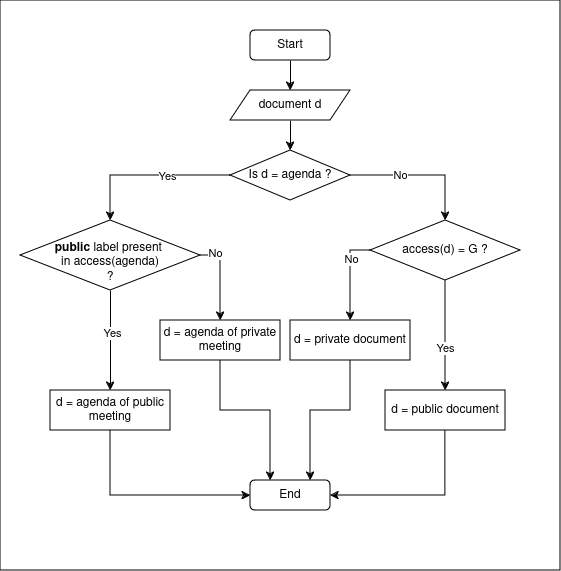
\includegraphics[width=0.8\textwidth]{./image/document_puclic_vs_private_classification.png}
    \caption{Process to identify whether a document is private or public}
    \label{fig:process to identify whether a document is private or public}
\end{figure} 

\noindent
Regarding other documents except agenda, for simplicity of implementation, we can include only \textbf{public} label in access control list, without including any other group of $\mathcal{G}$, to mean that $access(d) = \mathcal{G}$ or that document is a public document. Because, we do not need to include any other group ($g$) in a public non-agenda document, though we required them in public agenda documents for identifying meeting participants.\\ \\
\noindent
In addition to presence or absence of \textbf{public} label in $access(agenda)$, meeting agenda should define the \textbf{meeting quorum}, for the meeting. This theme will be discussed later.

% Definition of a meeting
\section{Definition of a meeting}

\noindent
\textbf{We assume that every meeting has an agenda associated with it, to define the set of groups($g$) required to attend the meeting}. Agenda of a particular meeting $M$ is a document, belonging to set $\mathcal{D}$.\\ \\
When we consider the agenda document of meeting $M$, for every group $g$ invited to meeting $M$; $g \in access(agenda)$. Also consider that, $D$ represents set of documents discussed in $M$, including agenda, such that $D \subseteq \mathcal{D}$. Hence, according to the assumption emphasized above, for any meeting $M$; $|D| \geq 1$.\\ \\ 
For conducting a meeting, at least 2 individuals are required. Consider that $I$ represents the set of individuals attending meeting $M$, such that $I \subseteq \mathcal{I}$, when groups ($g$) of $access(agenda)$ are converted to corresponding elementary individuals ($i$). Here we note that, for any meeting $M$; $|I| \geq 2$.\\
Accordingly, when $access(agenda)$ is defined in terms of singleton subsets of $\mathcal{G}$, and those groups (singleton subsets) in $access(agenda)$ are represented by $G$, such that $G \subseteq \mathcal{G}$, it can be observed that $|G| \geq 2$. \\ \\  
Consider set of locations of individuals in $M$ as $L$ (in other words, set of locations of individuals in set $I$, during meeting time), such that $L \subseteq \mathcal{L}$. Every individual attends meeting from a particular location $l$, such that $l \in L$. We note that, if meeting is online or hybrid, $|L| > 1$. If meeting is onsite, $|L| = 1$, since every individual is at same location. Every meeting should be in one mode, out of online, hybrid, onsite modes. Therefore, for any meeting $M$; $|L| \geq 1$. \\ \\
Since a \textbf{meeting} is a \textbf{synchronous} communication, every individual in meeting $M$ should attend the meeting during the same time slot $t$ (Assuming that all individuals are in same time zone).  \\ \\
Based on these definitions, we define meeting M as a 4-tuple,
    \[ M = < D, I, L, t > \]
such that,
    \[ D \subseteq \mathcal{D} \]
    \[ L \subseteq \mathcal{L} \]
    \[ I \subseteq \mathcal{I} \]
    \[ t \in \mathcal{T} \]


% Transformation of individual into role
\section{Transformation of individual into role}
\noindent
Consider that same sets defined above will be used in explanations below, in same notations: \\ \\
\noindent
Consider $g$ and $g'$ as subsets of $\mathcal{G}$ such that $g, g' \subseteq \mathcal{G}$. And consider $d$ as a \textbf{private} document , $l$ as a location and $t$ as a time slot such that $d \in \mathcal{D}$, $l \in \mathcal{L}$ and $t \in \mathcal{T}$.
Further consider that $g \in access(d)$ and $g' \notin access(d)$, for restricting access of document $d$, where $|access(d)| = n$ , given that $access(d)$ is defined as a set of singleton subsets of $\mathcal{G}$. A singleton subset of $\mathcal{G}$ means an elementary subset $g$, in which only one element (i.e. only one individual $i$) is present.\\ 
Also note that, $i$ and $i'$ are two individuals representing subsets $g$ and $g'$, respectively. \\ \\
\noindent
Assume that at scenario 1, $i$ attends a \textbf{meeting} at location $l$ during time slot $t$ to discuss document $d$, where $i'$ has no access to location $l$ during same time slot $t$. \\
Here we state that privacy of meeting discussing document $d$ was preserved at context $l \times t$ \\ \\ 
\noindent
Now assume that at scenario 2, $i$ attends a \textbf{meeting} at location $l$ during time slot $t$ to discuss document $d$, where $i'$ also has access to location $l$ during same time slot $t$. \\
Here we state that privacy of meeting discussing document $d$ was violated at context $l \times t$, because $n + 1$ individuals including $i'$ have got access to content of document $d$. But actually $|access(d)| = n$, when $access(d)$ is defined as a set of singleton subsets of $\mathcal{G}$, as mentioned above. We observe that $(n + 1) \geq |access(d)| = n$ \\ \\ 
\noindent
When above 2 scenarios are compared, we observe that role of same individual $i$, representing subset $g$ such that $g \in access(d)$, has experienced a variation. Context of $i$ has changed, depending on location and time. \\ \\
Therefore we define that presence of $i$ at context $l \times t$ transforms $i$ to role $r$.
\[ transform(i, l, t) = r : r \text{ is role of } i \text{ at location } l \text{ at time slot } t \] 
\noindent
If $g \in access(d)$, $g' \notin access(d)$ and $d$ is a \textbf{private} document, $i$ representing $g$ should attend a meeting to discuss $d$ at context $l \times t$, only if $i'$ representing $g'$ has no access to $l \times t$. Accordingly, to identify the privacy preserving context for discussing document $d$, combination of i, l, t is required.\\ \\



% Difference between public and private roles
\section{Difference between public and private roles}
When we consider a \textbf{private} document $d$, we can't exactly predict the time, at which $i'$, representing $g'$, such that $g' \notin access(d)$, will get access to location $l$. 
Therefore, meeting organizer has the responsibility of defining location $l$ as a \textbf{private} location or a \textbf{public} location, considering whether access of $i'$ has been strictly restricted, during all potential meeting time slots (represented by set $\mathcal{T}$).\\ \\
Using this definition and above formula, we can show that, $i$ representing $g$, such that $g \in access(d)$ where $d$ is a \textbf{private} document, is transformed to role $g$ itself, at a \textbf{private} location. 
Here, location should be defined as a \textbf{private} location, by same entity, that defined the set $access(d)$ for document $d$.

\[ transform(i, l, t) = r \]
\[ transform(i, (private\_location), t) = r \]
\[ transform(i, (private\_location), t) = g \] \\

\noindent
On the other hand, any location $l$ is defined as a \textbf{public} location, if access of $i'$ has \textbf{not} been strictly restricted, during any potential meeting time slot in set of time slots $\mathcal{T}$.\\ \\
Using this definition and above formula, we can show that, $i$ representing $g$, such that $g \in access(d)$, is transformed to \textbf{public} role, at a \textbf{public} location.
Location should be defined as a \textbf{public} location, by same entity, that defined the set $access(d)$ for document $d$.

\[ transform(i, l, t) = r \]
\[ transform(i, (public\_location), t) = r \]
\[ transform(i, (public\_location), t) = public \] \\
\noindent
Based on these derivations, we have identified a constraint relevant to $i$, for discussing $d$ in a privacy preserved meeting.\\ \\
\textbf{Constraint}: When $d$ is a \textbf{private} document, every $i$ representing $g$, such that $g \in access(d)$, that attends a meeting to discuss document $d$, must represent role $g$ in the meeting.\\ \\
When $d$ is a \textbf{public} document, every $i$ that attends a meeting to discuss document $d$, is allowed to represent \textbf{public} role in the meeting.\\ \\

% Sub-section: Roles in meeting agenda
\subsection{Roles in meeting agenda}
\noindent
If meeting agenda document does not include the group labeled as \textbf{public} in $access(agenda)$, it means that $\textbf{public} \notin access(agenda)$. Then $i'$ representing $g'$ such that $g' \notin access(d)$, should be strictly prevented from accessing the meeting, by conducting meeting at a \textbf{private} location, defined by relevant meeting organizing entity.\\ \\
On the other hand, if meeting agenda includes group labeled as \textbf{public} in $access(agenda)$, it means that $\textbf{public} \in access(agenda)$. Then it is \textbf{not} mandatory to prevent access of $i'$ representing $g'$ such that $g' \notin access(d)$, for the meeting. Therefore, meeting can be conducted at a \textbf{private} location or \textbf{public} location, based on locations defined by relevant meeting organizing entity.\\ \\

% Variation of role
\section{Variation of role}
\noindent
Now consider a situation where individual $i$ representing $g$, such that $g \in access(d)$ has $x$ number of locations, out of which any one can be selected for attending a meeting to discuss $d$. And assume that $i$ has $y$ number of time slots, out of which any one can be selected for attending the meeting.\\ \\
We can depict the possible variations of $transform(i, l, t)$ function as below, for individual $i$, depending on locations defined by the entity, assuming that $i$ doesn't change location during middle of a time slot.
\begin{table}[H]
    \centering
    \begin{tabular}{|c|c|c|c|c|c|}
    \hline
    $(i)$ & $t_1$ & $t_2$ & $...$ & $t_{y-1}$ & $t_{y}$ \\
    \hline
    $l_1$ & x & x & \  & x & x \\
    \hline
    $l_2$ & x & x & \  & x & x \\
    \hline
    $...$ & \  & \  & \  & \  & \  \\
    \hline
    $l_{x-1}$ & x & x & \  & x & x \\
    \hline
    $l_{x}$ & x & x & \  & x & x \\
    \hline
    \end{tabular}
    \caption{Possibilities in variation of $transform(i,l,t)$ for individual $i$}
    \label{tab:six_columns_six_rows}
\end{table}

\noindent
Note that $l_x$ represents the $x^{th}$ location, while $t_y$ represents the $y^{th}$ time slot. Meanwhile x represents the role of $i$ at the corresponding $l$ and $t$ (based on formula $transform(i, l, t) = r$). According to this representation, we observe that $i$ has $x \times y$ number of possibilities at maximum, to attain the role.\\ \\
Here we emphasize that some x roles can be categorized as \textbf{public}, with respect to \textbf{public} locations defined by an entity. According to the constraint identified, if $d$ is a \textbf{private} document, $i$ should attend the meeting only when $r = g$, such that $g \in access(d)$. When r = \textbf{public} role, individual $i$ should strictly avoid discussing \textbf{private} documents. By following this constraint, access of $i'$ representing $g'$, such that $g' \notin aceess(d)$, into this meeting can be prevented.\\ \\ 

% Meeting participant validation
\section{Privacy of documents}
\subsection{Participants in access control lists of non-agenda documents}
\noindent
It is possible to discuss one or more documents in a meeting. Further, there can be both public documents and private documents among these documents. We do not need to follow any constraint to protect the privacy of public documents.\\ \\
But when private documents are considered, it is needed to follow some constraints to protect the privacy. For example, consider $d_{1}$ and $d_{2}$ as 2 private documents. An individual $i$ representing $r$, such that $r = g$ and $g \in access(d_{1})$, can be absent in access control list of $d_{2}$. In other words, $g \notin access(d_{2})$ relationship can exist.\\ \\
In this situation, discussing both $d_{1}$ and $d_{2}$ in same meeting can violate the privacy of $d_{2}$, when above mentioned individual $i$ participates in that meeting. It means that, for discussing both $d_{1}$ and $d_{2}$ in same meeting, roles of all meeting participants should mandatorily be present in both $access(d_{1})$ and $access(d_{2})$. This relationship is graphically depicted in diagram below.
\begin{figure}[H]
    \centering
    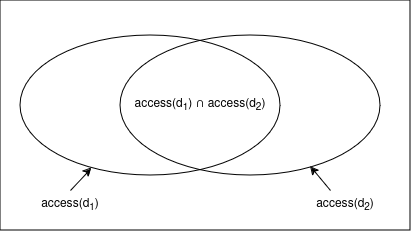
\includegraphics[width=0.7\textwidth]{./image/d1_intersection_d2.png}
    \caption{Intersection of access control lists of 2 private documents}
    \label{fig:intersection of access control lists of 2 private documents}
\end{figure} 
\noindent
This concept is applicable not only for 2 private documents, but also for any number of private documents discussed in same meeting. When there are $n$ number of private documents to discuss in a meeting, intersection of access control lists of all those documents should be considered. Any individual $i$ such that $i \notin (access(d_{1}) \cap access(d_{2}) \cap ... \cap access(d_{n-1}) \cap access(d_{n}))$ should be prevented from accessing the meeting.
\subsection{Meeting participant validation}
\noindent
When there are private documents to discuss in a meeting, it is required to validate intersection of participants identified as above, with participants included in access control list of meeting agenda (see "Meeting agenda" section for more details on meeting agenda).\\ 
For protecting privacy of $n$ number of private documents defined as $d_{1}, ... , d_{n}$, following relationship must be satisfied for the meeting. 
\[ access(agenda) \subseteq \{access(d_{1}) \cap access(d_{2}) \cap ... \cap access(d_{n-1}) \cap access(d_{n})\} \]
\noindent
Simply, above relationship means that each and every individual $i$ representing role $r$, such that $r = g$ and $g \in access(agenda)$, is also an element of the intersection of $access(d)$ of all private documents discussed in meeting.
A situation in which above relationship is violated can be explained by using following relationship. 
\[ \{access(d_{1}) \cap access(d_{2}) \cap ... \cap access(d_{n-1}) \cap access(d_{n})\} \subset access(agenda) \]
In simple terms, above relationship means that there exists at least one $i$ representing $r$, such that $r = g$ and $g \in access(agenda)$, where $g$ is not an element in the intersection of $access(d)$ of all private documents discussed in meeting.\\ \\
\noindent
However, for discussing public documents in meeting, it is not required to perform any participant validation. In other words, any individual $i$ can discuss public documents, in any private or public meeting.

% Privacy-preserved meeting
\section{Privacy-preserved meeting}
Based on above descriptions and definitions, we define privacy-preserved meeting as below;\\ \\
\textbf{A privacy-preserved meeting is a meeting in which, individual i representing role r has no access to the meeting, when $r = g$ and $g \notin access(agenda)$, where access(agenda) satisfies,} 
\[access(agenda) \subseteq \{access(d_{1}) \cap access(d_{2}) \cap ... \cap access(d_{n-1}) \cap access(d_{n})\} \]
\textbf{for all private documents $d_{1} ... d_{n}$, discussed in the meeting.} 

% Meeting quorum
\section{Meeting quorum}
\noindent
In a \textbf{privacy-preserved meeting} of our research context, we define \textbf{meeting quorum} as the minimum number of individuals ($i$) representing participant groups ($g$), required to attend a meeting, such that $g \in access(agenda)$. \\ \\
In privacy preserved meeting context, if a specific \textbf{meeting quorum} rule is not defined in the agenda, other than $access(agenda)$ set, we assume that every $i$ such that, 
\begin{itemize}
    \item $i \in g$, and
    \item $g \in access(agenda)$, 
\end{itemize}
\noindent
is required for the meeting. But, it is not applicable for $g = \textbf{public}$. In such a situation, when a numeric meeting quorum rule is not defined specifically, $|meeting\ quorum| = |access(agenda)|$, where $access(agenda)$ is defined in form of singleton subsets of $\mathcal{G}$. \\ \\
\noindent
In addition, it is possible that $|meeting\ quorum| < |access(agenda)|$, if a numeric \textbf{meeting quorum} rule is defined in meeting agenda. Therefore in overall, $|meeting\ quorum| \leq |access(agenda)|$, when $access(agenda)$ is defined in form of singleton subsets of $\mathcal{G}$. \\ \\
Since at least 2 individuals ($i$) are required for any meeting, $2 \leq |meeting\ quorum|$. \\ \\
Accordingly, $2 \leq |meeting\ quorum| \leq |access(agenda)|$. \\ \\
When $access(agenda)$ is defined in form of singleton subsets of $\mathcal{G}$, as we have already depicted earlier, $|access(agenda)| \leq |\mathcal{I}|$. By merging this inequality with above expression, we obtain following expression theoretically.\\ \\
$2 \leq |meeting\ quorum| \leq |access(agenda)| \leq |\mathcal{I}|$  \\ \\

% Problem analysis
\section{Problem analysis}
Our problem focused in organizing privacy-preserved meetings has few distinct steps, that can be clearly identified within it. Based on decision making points identified within the problem, this problem was mapped into a boolean circuit, following a union operation. Here, union operation can be introduced as a set related pre-processing operation, applied on the $access(d)$ sets of all documents of the meeting, including the $agenda$. Before applying this union operation, it is needed to make sure that, all groups except the $public$ group in those $access(d)$ sets are converted to singleton groups. Distinct sections of the problems are analyzed below, considering the circuit diagrams produced for them.\\ \\
% Participant validation based on documents
\subsection{Participant validation based on documents}
After calculating the union of $access(d)$ sets of all documents to be discussed in the meeting, as $access(doc\_1) \cup ... \cup access(doc\_n)\} \cup access(agenda)$, $public$ group is subtracted, since our initial requirement is to identify all the individuals having access to at least one document. In addition, we identify all documents associated with meeting as $doc\_1, ..., doc\_n, agenda$, since we need to check whether each individual in the union of individuals identified, has access to all the documents, for discussing them in a meeting. In example depicted in the diagram, consider that there are only 3 individuals as $i\_1, i\_2, i\_3$ and only 4 documents as $doc\_1, doc\_2, doc\_3, agenda$.\\ \\
Algorithm for participant validation section is explained below.
\begin{algorithm}[H]
    \caption{Participant validation based on documents}
    \begin{algorithmic}[1]
        \State \textbf{Input:} Access control lists (access(d)) of documents \(doc\_1\), ... , \(doc\_n\), \(agenda\)
        \State \textbf{Output:} Eligibility of each individual for meeting by document analysis \\
        \State union of \(access(d)\) = \(access(doc\_1) \cup \dots \cup access(doc\_n) \cup access(agenda)\)
        \State union of individuals = union of \(access(d) - public \)
        \State set of documents = \(doc\_1, \dots , doc\_n , agenda\)
        \For{each individual \(i\_n\) in (union of individuals)}
            \State validity of \(i\_n\) by doc analysis = true
            \For{each \(doc\_x\) in (set of documents)}
                \If{\(doc\_x \neq agenda\)}
                    \State validity of \(i\_n\) for \(doc\_x\) = \((i\_n \in access(doc\_x)) \text{ OR } (public \in access(doc\_x))\)
                \Else
                    \State validity of \(i\_n\) for \(doc\_x\) = \(i\_n \in access(agenda)\)
                \EndIf
                \State validity of \(i\_n\) by doc analysis = validity of  \(i\_n\) by doc analysis \(\text{ AND validity of } i\_n\) for \(doc\_n\)
            \EndFor
            \State \textbf{Return} validity of \(i\_n\) by doc analysis
        \EndFor
    \end{algorithmic}
\end{algorithm}
Above algorithm explains the process depicted by logical circuit diagram below. In the algorithm, 
\[|union\ of\ access(d)| = |access(doc\_1)| + ... + |access(doc\_n)| + |access(agenda)| \]
relationship means that time complexity of the $union\ of\ access(d)$ operation is, $O(|access(doc\_1)| + ... + |access(doc\_n)| + |access(agenda)|)$. It is a linearly increasing time complexity. In addition, each iteration in outer loop outputs whether an individual of the union of individuals is valid by $access(d)$ analysis of all documents. Inner loop checks whether particular individual has access to all documents including $agenda$. Operations within the loops are considered as operations of constant time complexity, $O(1)$. Accordingly, since there is a nested loop in above algorithm, time complexity of this section of problem can be $O(n^{2})$, at maximum. Because number of individuals can be any positive integer, and number of documents including $agenda$ also can be any positive integer. 

\begin{figure}[H]
    \centering
    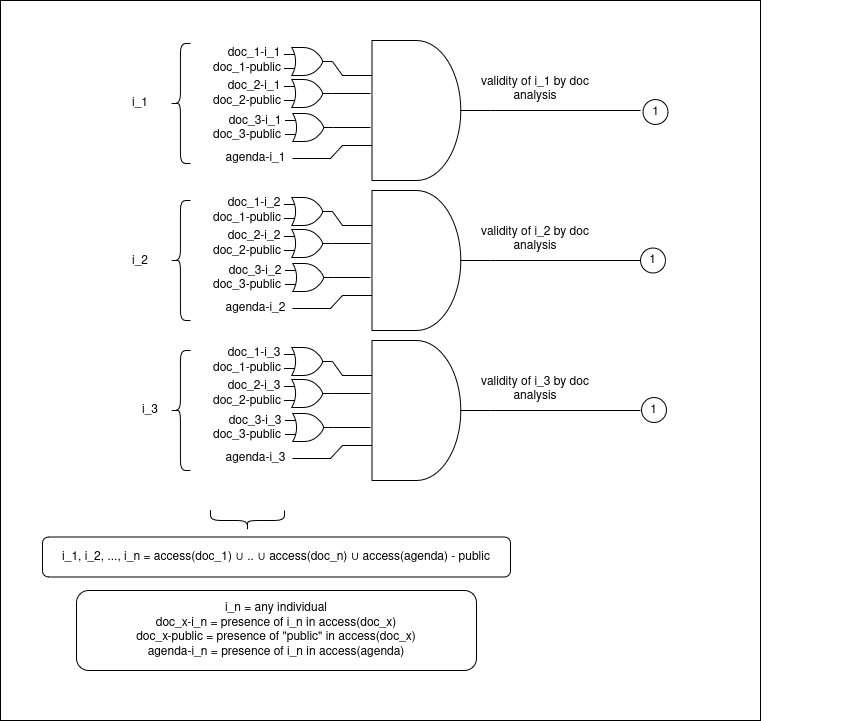
\includegraphics[width=0.9\textwidth]{./image/circuit_diagram/1_participant_validation.png}
    \caption{Participant validation based on $access(d)$ of documents}
    \label{fig:participant validation based on documents}
\end{figure} 

% Meeting quorum satisfiability of time slots
\subsection{Meeting quorum satisfiability of time slots}
\subsubsection{Eligibility of each individual, in each time slot, for meeting}
After checking the validity of each participant by document analysis, it is needed to check their locations in different time slots. Based on the location, eligibility of each individual to discuss the set of documents changes. Because, as we have described earlier, $private$ documents should be discussed at $private$ locations only, while $public$ documents can be discussed at any location. If there is at least one $private$ document in the set of documents discussed in meeting, then each individual $i\_n$ validated by document analysis should attend this meeting from a $private$ location. Following circuit diagram consists of the location analysis of each individual, in every time slot. Here, these time slots mean the time slots belonging to the union of available time slots of all individuals, present in the union of individuals, mentioned in previous algorithm.\\ \\ 
For deciding the eligibility of each individual, to discuss set of documents, in different time slots, we need inputs included in the following table. In it, each individual of the union of individuals, and his/her available time slots with locations should be present. Please note that following table consists of some sample data only, as individuals, time slots and locations. It is supposed to contain the real data, regarding the respective scenario. For simplicity, we consider only 3 locations as onsite, remote\_private and remote\_public, since every location can be categorized into one of those 3 categories, by a meeting organizing entity.\\ \\
\begin{table}[H]
    \centering
    \begin{tabular}{|c|c|c|}
    \hline
    Individual $(i\_x)$ & Time slot(slot$y$) & Location \\
    \hline
    $i\_1$ & slot1 & onsite \\
    \hline
    $i\_1$ & slot2 & remote\_private \\
    \hline
    $i\_1$ & slot3 & remote\_public \\
    \hline
    ... & ... & ... \\
    \hline
    $i\_n$ & slot$m$ & location of $i\_n$ in slot$m$ \\
    \hline
    \end{tabular}
    \caption{Available time slots and locations of individuals, in union of individuals}
    \label{tab:three_columns_six_rows}
\end{table}

Algorithm for deciding the eligibility of each individual, to discuss the set of documents of meeting, in different time slots, is described below.\\ \\
\begin{algorithm}[H]
    \caption{Deciding eligibility of each individual for meeting, in each time slot}
    \begin{algorithmic}[1]
        \State \textbf{Input 1:} Validity of each individual \(i\_1\), ... , \(i\_n\) by doc analysis
        \State \textbf{Note:} Individuals \(i\_1\), ... , \(i\_n\) mean union of individuals of previous algorithm, and \textbf{input 1} is obtained from output of previous algorithm
        \State \textbf{Input 2:} Availability of each individual in each time slot (at any location) 
        \State \textbf{Input 3:} Location of each individual in each time slot (whether remote\_public or no)
        \State \textbf{Note:} \textbf{Input 2} and \textbf{input 3} are obtained from the table containing available time slots and locations of individuals.
        \State \textbf{Input 4:} Presence of \(public\) group in \(access(d)\) of each document, in set of documents, as $(doc\_1-public) , ... , (doc\_n-public) , (agenda-public)$
        \State \textbf{Output:} Eligibility of each individual, to discuss the set of documents, in each time slot \\
        \State union of time slots = \(availability(i\_1) \cup \dots \cup availability(i\_n)\)
        \For{each slot\_\(x\) in (union of time slots)}
            \For{each individual \(i\_y\) in (union of individuals)}
                \State publicity of meeting = \((doc\_1-public) \text{ AND } ... \text{ AND } (doc\_n-public) \text{ AND } (agenda-public)\)
                \State slot\(\_x-i\_y\) = availability of \(i\_y\) in slot\_\(x\) at any location
                \State slot\(\_x-i\_y\)\_remote\_public = whether \(i\_y\) is at remote\_public location in slot\_\(x\) 
                \State availability of slot\(\_x-i\_y\) for public meeting = (publicity of meeting) AND (slot\(\_x-i\_y\))
                \State availability of slot\(\_x-i\_y\) for private meeting = (slot\(\_x-i\_y\)) AND NOT(slot\(\_x-i\_y\)\_remote\_public)
                \State availability of slot\(\_x-i\_y\) for meeting by time slot analysis = (availability of slot\(\_x-i\_y\) for public meeting) OR (availability of slot\(\_x-i\_y\) for private meeting)
                \State slot\(\_x-i\_y\) eligibility for meeting = (Validity of \(i\_y\) by doc analysis) AND (availability of slot\(\_x-i\_y\) for meeting by time slot analysis)
            \EndFor
            \State \textbf{Return} slot\(\_x-i\_y\) eligibility for meeting
        \EndFor
    \end{algorithmic}
\end{algorithm}
In above algorithm, time complexity of $union\ of\ time\ slots$ operation is,\\ $O(|availability(i\_1)| + \dots + |availability(i\_n)|)$, at maximum. It is a linear time complexity. When considering the loops, outer loop iterates through all time slots, in the union of time slots, calculated by considering available time slots of all individuals, in union of individuals. Meanwhile, inner loop iterates through each individual in the union of individuals. In addition, number of documents discussed in the meeting can be any positive integer. Number of documents is considered when deciding the meeting publicity, within the inner loop. Further, validity of the individual by document analysis, obtained from output of previous algorithm, is utilized in in inner loop. Number of documents is concerned for that as well. But, it is in parallel level, with publicity calculation of the meeting. Therefore, we can consider that number of documents has linear time complexity as $O(n)$, within inner loop. Accordingly, it is observed that, time complexity of above algorithm can be $O(n^{3})$, at maximum, due to outer loop, inner loop, and number of documents within inner loop.\\ \\
Circuit diagram corresponding to above algorithm is depicted below. The following boolean circuit is supposed to be repeated for each individual, in each time slot, as explained in algorithm.
\begin{figure}[H]
    \centering
    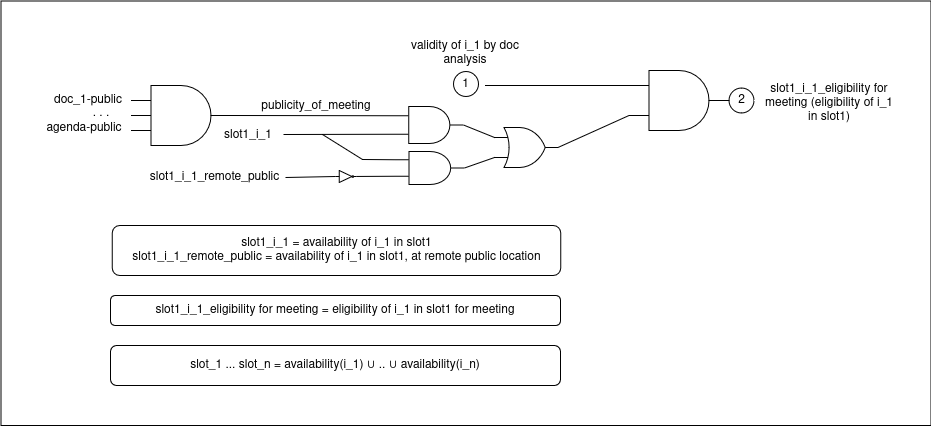
\includegraphics[width=0.9\textwidth]{./image/circuit_diagram/2_slot_n_i_n_eligibility.png}
    \caption{Eligibility of each individual for meeting, in each time slot}
    \label{fig:eligibility of each individual for meeting, in each time slot}
\end{figure} 

\subsubsection{Meeting quorum satisfiability}
Eligibility of each individual to discuss the set of documents, in each time slot, is considered for deciding the quorum satisfiability of each time slot, in the union of time slots. Then it is checked whether there is at least one quorum satisfying time slot. Because, if there is no at least one quorum satisfying time slot, then it is not possible to conduct the meeting.\\ \\
Algorithm for checking the quorum satisfiability of time slots is explained below.
\begin{algorithm}[H]
    \caption{Identifying meeting quorum satisfiability of time slots}
    \begin{algorithmic}[1]
        \State \textbf{Input 1:} Eligibility of each individual for meeting, in each time slot
        \State \textbf{Note:} \textbf{Input 1} is obtained from output of previous algorithm
        \State \textbf{Input 2:} Numerical meeting quorum value 
        \State \textbf{Input 3:} Availability of each individual in each time slot (at any location)
        \State \textbf{Output:} Existence of quorum satisfying time slot/s, for the meeting \\
        \State union of time slots = \(availability(i\_1) \cup \dots \cup availability(i\_n)\)
        \State availability of a meeting quorum satisfying time slot = false
        \For{each slot\_\(x\) in (union of time slots)}
            \State meeting quorum satisfiability of slot\_\(x\) = false
            \State combinations of individuals in slot\_\(x\) = combinations of individuals, with magnitude of meeting quorum size 
            \For{each \(combination\) in (combinations of individuals in slot\_\(x\))}
                \State meeting quorum satisfiability of \(combination\) = AND operation (for all individuals in the \(combination\))
                \State meeting quorum satisfiability of slot\_\(x\) = (meeting quorum satisfiability of slot\_\(x\)) OR (meeting quorum satisfiability of \(combination\))
            \EndFor
            \State \textbf{Return} availability of a meeting quorum satisfying time slot = (availability of a meeting quorum satisfying time slot) OR (meeting quorum satisfiability of slot\_\(x\))
        \EndFor
    \end{algorithmic}
\end{algorithm}
Similar to previous algorithm, in above algorithm also, time complexity of $union\ of\ time\ slots$ operation is, $O(|availability(i\_1)| + \dots + |availability(i\_n)|)$, at maximum. It is observed that, in loop structure, outer loop iterates through all time slots in union of time slots. That number of time slots can be any positive integer. Inner loop contains a $combination$ operation, which is intended to create combinations of magnitude of meeting quorum size, out of individuals of the union of individuals. Mathematically, number of such possible combinations can be calculated as,
\[ n \text{C} r = \binom{n}{r} = \frac{n!}{r!(n-r)!} \]
when n = number of individuals in union of individuals, and r = meeting quorum size.\\ \\
Regarding $combination$ operation, highest number of combinations is obtained when $r = \frac{n}{2}$ or $r \approx \frac{n}{2}$ (\ref{proof: maximum value of ncr when n is n/2}). Number of possible combinations reduces, when $r$ is considerably small ($r \approx 0$), or when $r$ is close to $n$ ($r \approx n$). Due to this nature of $combination$ operation, maximum possible time complexity for creating $n \text{C} r$ number of combinations is $O\binom{n}{\frac{n}{2}}$ or $O\binom{n}{\frac{n-1}{2}}$, depending on whether $n$ is even or odd.\\ \\
In the inner loop of above algorithm, since AND operation is applied for all individuals, in each $combination$ created, maximum time complexity associated with inner loop is $O(n \text{ x } \binom{n}{\frac{n}{2}})$ or $O(n \text{ x } \binom{n}{\frac{n-1}{2}})$. Because the number of individuals in each combination created, or the meeting quorum size, can be any positive integer. In addition, since inner loop is repeated by outer loop, where number of time slots also can be any positive integer, maximum possible time complexity of above algorithm is, 
\[O(n \text{ x } n \text{ x } \binom{n}{\frac{n}{2}}) = O(n^{2} \text{ x } \binom{n}{\frac{n}{2}}) \text{ ,when union has even number of individuals} \]
\[ \text{or} \]
\[O(n \text{ x } n \text{ x } \binom{n}{\frac{n-1}{2}}) = O(n^{2} \text{ x } \binom{n}{\frac{n-1}{2}}) \text{ ,when union has odd number of individuals.} \]\\

Time complexity of $O(n^{2} \text{ x } \binom{n}{\frac{n}{2}})$ or $O(n^{2} \text{ x } \binom{n}{\frac{n-1}{2}})$ has polynomial component of $O(n^{2})$. Further, when considering $O\binom{n}{\frac{n}{2}}$ or $O\binom{n}{\frac{n-1}{2}}$ component, it is observed that, for large $n$ values, 
\[ O\binom{n}{\frac{n}{2}} \approx O(\frac{2^{n}}{\sqrt{n}}) \ \ \ \ \ \ref{proof: time complexity of nc(n/2)} \] 
\[ \text{or} \]
\[ O\binom{n}{\frac{n-1}{2}} \approx O(\frac{2^{n}}{\sqrt{n}}) \ \ \ \ \ \ref{proof: time complexity of nc((n-1)/2)} \] 
depending on whether union has an even number of individuals, or an odd number of individuals.\\

Time complexity of $O(\frac{2^{n}}{\sqrt{n}})$ has $O(2^{n})$ as the dominant term, for large values of $n$. Time complexity $O(2^{n})$ is considered as a non-polynomial time complexity, because $n$ is not a constant value (\cite{pfleeger1996chapter3}). Since non-polynomial time complexity of $O(2^{n})$ increases exponentially with increase of $n$, it is eligible to use a heuristic or an existing library, when implementing above algorithm for execution with inputs. Because, there is no specific standard methodology defined, for creating combinations, as included in above algorithm.\\ \\
Figure below depicts the corresponding boolean circuit for above algorithm.\\ \\

\begin{figure}[H]
    \centering
    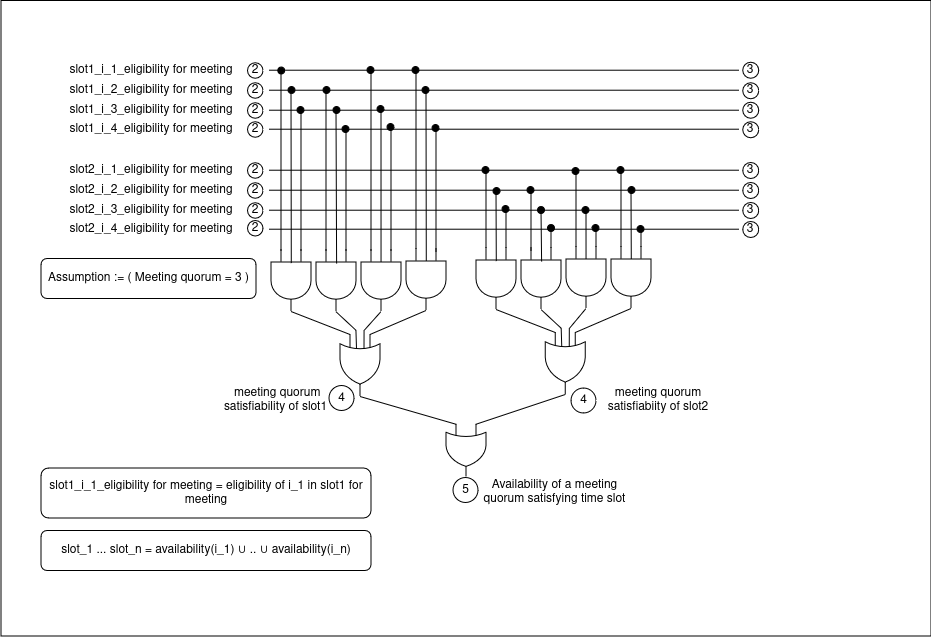
\includegraphics[width=0.9\textwidth]{./image/circuit_diagram/3_quorum_satisfying_slot_selection.png}
    \caption{Meeting quorum satisfiability of time slots}
    \label{fig:meeting quorum satisfiability of time slots}
\end{figure} 

% Earliest time slot selection
\subsection{Selection of earliest, meeting quorum satisfying time slot}
Selecting the earliest, meeting quorum satisfying time slot is not required to find a solution for our research problem. Because, after identifying the quorum satisfying time slots by above algorithm, our next objective associated with research problem is to, analyze the privacy-preserving meeting mode for each meeting quorum satisfying time slot. Therefore, we introduce this step of selecting the earliest, meeting quorum satisfying time slot, as an additional step provided by us. Since privacy-preserved meeting organization is a real world problem, when implementing a usable system for that purpose, this additional step can be helpful to identify the earliest, eligible time slot for conducting the privacy-preserved meeting, rather than suggesting numerous eligible time slots.\\ \\
Algorithm for selecting the earliest, meeting quorum satisfying time slot is explained below.\\ \\
\begin{algorithm}[H]
    \caption{Selection of earliest, meeting quorum satisfying time slot}
    \begin{algorithmic}[1]
        \State \textbf{Input:} Meeting quorum satisfiability of time slots, in union of time slots
        \State \textbf{Note:} \textbf{Input} is produced by processing previous algorithm
        \State \textbf{Output:} Earliest, meeting quorum satisfying time slot \\
        \State union of time slots with quorum satisfiability = quorum satisfiability of each time slot, in \((availability(i\_1) \cup \dots \cup availability(i\_n))\), in the order of precedence
        \State earliest eligible time slot = initialization of an empty list type structure, to store whether each slot is earliest eligible slot or no
        \For{each slot\_\(x\) and \(meeting\_quorum\_satisfiability\) in (union of time slots with quorum satisfiability)}
            \If{slot\_\(x\) is earliest slot in (union of time slots with quorum satisfiability)}
                \State store slot\_\(x\) and its \(meeting\_quorum\_satisfiability\), in (earliest eligible time slot) list     
            \Else
                \State previous condition = list to store result of, NOT operation (for each slot currently stored in (earliest eligible time slot) list)
                \State previous condition integrated = AND operation (for all slots in (previous condition) list) 
                \State whether slot\_\(x\) is earliest meeting quorum satisfying time slot = ((\(meeting\_quorum\_satisfiability\) of slot\_\(x\) = true) AND ((previous condition integrated) = true))
                \State store slot\_\(x\) and (whether slot\_\(x\) is earliest meeting quorum satisfying time slot), in (earliest eligible time slot) list                
            \EndIf
        \EndFor
        \State \textbf{Return} (earliest eligible time slot) list 
        \State \textbf{Note:} At \textbf{Return} point, (earliest eligible time slot) list contains \(true\) for earliest, meeting quorum satisfying time slot, and \(false\) for all other time slots
    \end{algorithmic}
\end{algorithm}

In above algorithm, there is a reason to apply a different process on the earliest time slot in union of time slots, apart from all other time slots in the union. If earliest time slot in union of time slots satisfies the meeting quorum, then without considering any pre-condition, it becomes the earliest meeting quorum satisfying time slot. It can be analyzed by extracting it as a separate condition, like below. \\ \\
\textbf{If} earliest slot in union of time slots satisfies the meeting quorum, \textbf{Then} \\
\indent earliest slot is the earliest, meeting quorum satisfying time slot \\
\textbf{Else}\\
\indent earliest slot is \textbf{not} the earliest, meeting quorum satisfying time slot \\
\textbf{End If}  \\ \\
Above condition block is the meaning implied by "If" block, in the condition of the algorithm. But, if any time slot other than the earliest time slot of union, satisfies the meeting quorum, then it is needed to check an additional condition as well, to identify whether it is the \textbf{earliest} meeting quorum satisfying time slot or no. Accordingly, following condition block elaborates the meaning implied by "Else" block of the condition, in above algorithm. \\ \\             
\textbf{If} any slot$x$ which is \textbf{not} the earliest slot in union of time slots, satisfies the meeting quorum, \textbf{Then} \\
\indent \textbf{If} any earlier slot than slot$x$ does \textbf{not} satisfy the meeting quorum, \textbf{Then} \\
\indent \indent slot$x$ is the earliest, meeting quorum satisfying time slot \\
\indent \textbf{End If}\\
\textbf{Else}\\
\indent slot$x$ is \textbf{not} the earliest, meeting quorum satisfying time slot \\
\textbf{End If}  \\ \\
It is observed that, there is a nested "If" condition in "If" block, in above condition block. Requirement to check this additional condition, is the reason for treating earliest time slot in union of time slots in a different manner, than other time slots, when identifying the earliest meeting quorum satisfying time slot.\\ \\
Above algorithm utilizes the meeting quorum satisfiability of each time slot, obtained by processing previous algorithm. Therefore, When we calculate the time complexity of above algorithm, we consider that meeting quorum satisfiability information is stored in an eligible data structure after processing previous algorithm. Otherwise, if we consider these both algorithms together, time complexity of above algorithm and previous algorithm collectively becomes, $O(2^{n})$ at maximum, as explained in time complexity description of previous algorithm.\\ \\
But, when meeting quorum satisfiability information obtained from previous algorithm is stored in an eligible data structure and provided to above algorithm, time complexity of above algorithm is dominated by "for" loop, and its content. Number of iteration in this loop can be any positive integer. There is no inner loop, in the "for" loop. But, in "Else" block of each iteration, "NOT" operation is applied on each time slot, until the slot which is currently being iterated by "for" loop. Therefore, it is observed that, time complexity of above algorithm can be $O(n^{2})$, at maximum. Even though there is an "AND" operation applied on all time slots, in the "Else" block, it can be neglected, when calculating time complexity. Because, it is in the parallel level to "NOT" operation, which is already considered. All other operations within above algorithm are considered as operations having constant time complexity.\\ \\
Circuit diagram corresponding to above algorithm is depicted below.\\ \\

\begin{figure}[H]
    \centering
    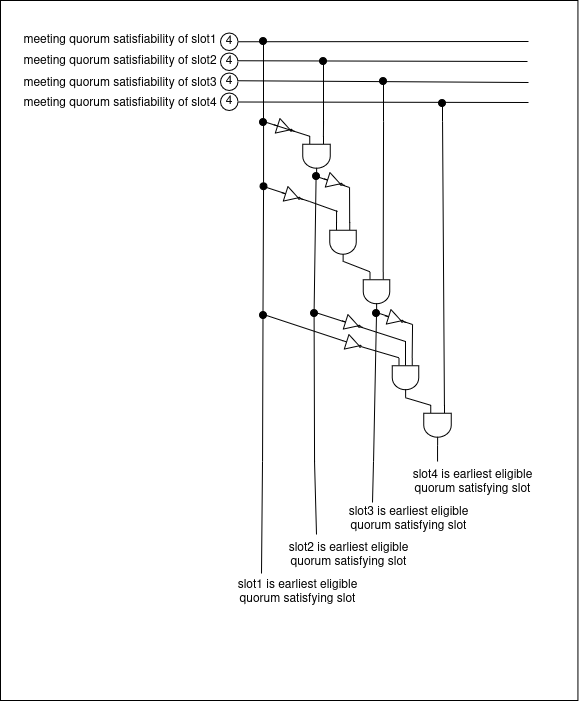
\includegraphics[width=0.9\textwidth]{./image/circuit_diagram/4_earliest_slot_selection.png}
    \caption{Selection of earliest, meeting quorum satisfying time slot}
    \label{fig:selecting earliest, meeting quorum satisfying time slot}
\end{figure} 

% Meeting mode selection
\subsection{Meeting mode selection} \label{sec:logic_for_selecting_the_meeting_mode}
After identifying the quorum satisfying time slots, meeting mode of each time slot should be decided, based on locations of eligible participants. In real world scenario, participants can be present at numerous locations. However in our research, as it is already mentioned earlier, only three location types are considered (onsite, remote\_private and remote\_public locations). It is observed that three meeting modes are possible, based on those three locations, as onsite mode, hybrid mode and online mode. Logic for deciding the meeting mode is depicted by the flow chart below.
\begin{figure}[H]
    \centering
    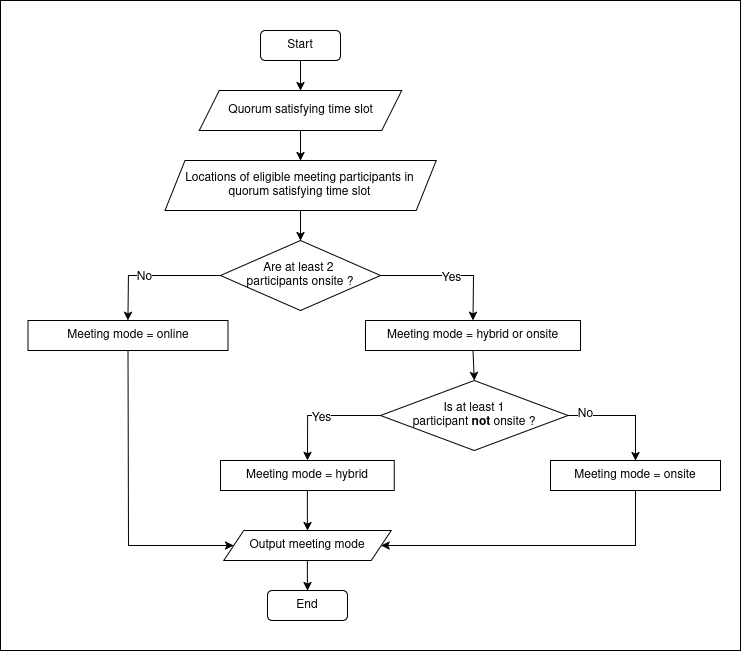
\includegraphics[width=0.9\textwidth]{./image/meeting_mode_selection.png}
    \caption{Logic for selecting the meeting mode}
    \label{fig:logic for selecting the meeting mode}
\end{figure} 
According to the logic, initially we check whether at least two eligible participants are at onsite locations, during the quorum satisfying time slot. If only one participant is at onsite location (i.e. onsite office location of meeting organization), or no one is at onsite location, it means that obviously meeting will be in online mode. But, if at least two participants are available at onsite location, it is required to check whether at least one participant is not at the onsite location. If at least one participant is at a remote location in the considered time slot, meeting will obviously be in hybrid mode. Unless, if at least two participants are onsite and, at least one participant is \textbf{not} at a remote location (remote\_private or remote\_public), it means that all available participants are at onsite location. It implies that meeting is in onsite mode.\\ \\
The algorithm for deciding the meeting mode of quorum satisfying time slot is explained below.\\ \\
\begin{algorithm}[H]
    \caption{Meeting mode selection}
    \begin{algorithmic}[1]
        \State \textbf{Input 1:} Eligibility of each participant for meeting, in each time slot
        \State \textbf{Note:} \textbf{Input 1} is produced by processing algorithm 1
        \State \textbf{Input 2:} Meeting quorum satisfiability of each time slot, in union of time slots
        \State \textbf{Note:} \textbf{Input 2} is produced by processing algorithm 3
        \State \textbf{Input 3:} Whether each meeting participant is at onsite location, in each time slot
        \State \textbf{Output:} Whether meeting mode is onsite or hybrid or online \\

        \For{each slot\_\(x\) in (union of time slots)}
            \State slot\_\(x\) onsite = initialize an empty list
            \State slot\_\(x\) online = initialize an empty list
            \For{each participant\_\(y\) with \(eligibility\ for\ meeting\) status in slot\_\(x\)}
                \State participant\_\(y\)\_slot\_\(x\)\_onsite = whether participant\_\(y\) is onsite in slot\_\(x\)
                \State append to (slot\_\(x\) onsite) list: (\(eligibility\ for\ meeting\) for participant\_\(y\)) AND (participant\_\(y\)\_slot\_\(x\)\_onsite)
                \State append to (slot\_\(x\) online) list: (\(eligibility\ for\ meeting\) for participant\_\(y\)) AND NOT(participant\_\(y\)\_slot\_\(x\)\_onsite)
            \EndFor
            \State slot\_\(x\) is onsite or hybrid = false
            \State onsite combinations of slot\_\(x\) = create all possible combinations of size 2, with items in (slot\_\(x\) onsite) list
            \For{each combination\_\(z\) in (onsite combinations of slot\_\(x\))}
                \State combination\_\(z\) is onsite = apply AND operation between 2 items in combination\_\(z\)
                \State slot\_\(x\) is onsite or hybrid = (slot\_\(x\) is onsite or hybrid) OR (combination\_\(z\) is onsite)
            \EndFor
            \State \textbf{eligibility of slot\_\(x\) for online mode} = (NOT(slot\_\(x\) is onsite or hybrid)) AND (meeting quorum satisfiability of slot\_\(x\))
            \State slot\_\(x\) is hybrid = false
            \For{each participant \(p\) in (slot\_\(x\) online) list}
                \State slot\_\(x\) is hybrid = (slot\_\(x\) is hybrid) OR (whether participant \(p\) is online)
            \EndFor
            \State \textbf{eligibility of slot\_\(x\) for hybrid mode} = (slot\_\(x\) is hybrid) AND \{(meeting quorum satisfiability of slot\_\(x\)) AND (slot\_\(x\) is onsite or hybrid)\}
            \State \textbf{eligibility of slot\_\(x\) for onsite mode} = (NOT(slot\_\(x\) is hybrid)) AND \{(meeting quorum satisfiability of slot\_\(x\)) AND (slot\_\(x\) is onsite or hybrid)\}
            \State \textbf{Return} eligibility of slot\_\(x\) for online mode, eligibility of slot\_\(x\) for hybrid mode, eligibility of slot\_\(x\) for onsite mode
            \State \textbf{Note:} At \textbf{Return} point, depending on whether eligible meeting mode is online or hybrid or onsite, respective variable will be \textbf{true}, and other two variables will be \textbf{false}.
        \EndFor
    \end{algorithmic}
\end{algorithm}
When considering the algorithm above, it is observed that it obtains multiple outputs from previous algorithms. In other words, it is impossible to provide inputs required by this algorithm, without processing previous algorithms. However, since it is not mandatory to execute this algorithm in parallel with previous algorithms, it is possible to calculate the the time complexity of this algorithm, as below.\\ \\
In above algorithm, it is observed that there is a nested "for" loop structure. There are some separate"for" loops, inside the outer loop. Among those "for" loops, the loop iterating through all possible combinations of two individuals has $n \text{C} r$ number of iterations, where $n$ = number of individuals in union of individuals, and r = 2. Therefore, maximum possible number of iterations in that particular inner loop can be mathematically calculated as below. 
\[ n \text{C} 2 = \binom{n}{2} = \frac{n!}{2!(n-2)!} \]
\[ \frac{n!}{2!(n-2)!} = \frac{n!}{2 \text{ x } (n-2)!} \]
\[ \frac{n!}{2 \text{ x } (n-2)!} = \frac{{(n-2)! \text{ x } (n-1) \text{ x } n}}{2 \text{ x } (n-2)!} \]
\[ \frac{{(n-2)! \text{ x } (n-1) \text{ x } n}}{2 \text{ x } (n-2)!} = \frac{(n-1) \text{ x } n}{2} \]
\[ \therefore n \text{C} 2 = \frac{(n-1) \text{ x } n}{2} = \frac{n^2}{2} - \frac{n}{2} \]
Maximum possible time complexity of "for" loop, which iterates through all possible combinations of two individuals is $O(n \text{C} r)$. Since value of r = 2, and depending on above calculation, time complexity of this "for" loop can be depicted as below.\\ \\
\[ O(n \text{C} 2) = O(\frac{n^2}{2} - \frac{n}{2}) \]
In addition, when considering the outer "for" loop together with the inner "for" loop, that iterates through all possible combinations of two individuals, total time complexity can be calculated as below. Because, outer loop can iterate through $n$ number of iterations, where $n$ can be any positive integer.\\ \\
\[ O(n) \text{ x } O(n \text{C} 2) = O(n \text{ x } (n \text{C} 2)) \]
\[ O(n \text{ x } (n \text{C} 2)) = O(n \text{ x } (\frac{n^2}{2} - \frac{n}{2})) \]
\[ O(n \text{ x } (\frac{n^2}{2} - \frac{n}{2})) = O(\frac{n^3}{2} - \frac{n^2}{2}) \]
\[ O(\frac{n^3}{2} - \frac{n^2}{2}) = O(\frac{n^2(n - 1)}{2}) \]
Except above discussed inner "for" loop that iterates through combinations, every other inner "for" loop can iterate through $n$ number of iterations, where $n$ is any positive integer. When such a "for" loop is considered together with the outer "for" loop, which also can iterate thorugh $n$ number of iterations, combined time complexity becomes $O(n \text{ x } n)$. It can be simplified as below.\\ \\
\[ O(n \text{ x } n) = O(n^2) \] 
Accordingly, maximum possible time complexity of above algorithm can be either $O(\frac{n^2(n - 1)}{2})$ or $O(n^2)$, depending on situation. When $n > 3$, maximum time complexity of above algorithm is $O(\frac{n^2(n - 1)}{2})$. When $n = 3$, $O(\frac{n^2(n - 1)}{2}) = O(n^2)$. In addition to those two cases, when positive integer $n$ satisfies $n < 3$ condition, maximum time complexity is $O(n^2)$.\\ \\
The circuit diagram corresponding to the above algorithm is depicted by figure below.\\ \\
\begin{figure}[H]
    \centering
    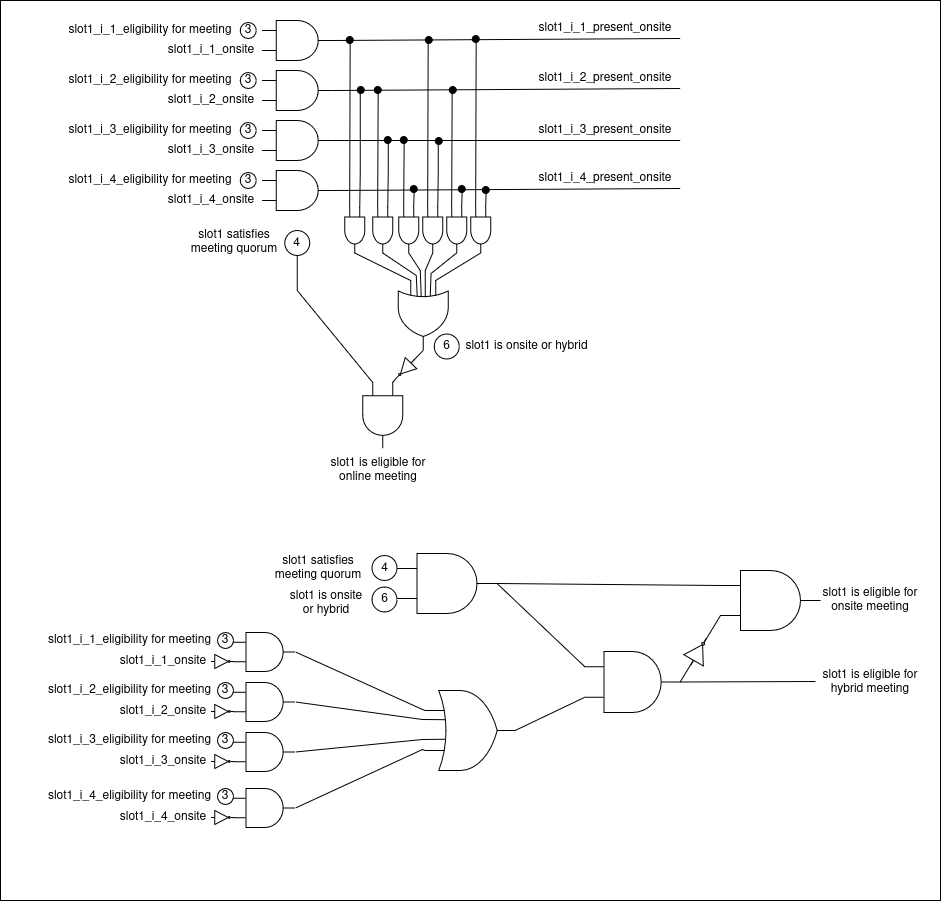
\includegraphics[width=0.9\textwidth]{./image/circuit_diagram/5_meeting_mode_selection.png}
    \caption{Circuit diagram for selecting the meeting mode}
    \label{fig:circuit diagram for selecting the meeting mode}
\end{figure}

% Complexity if the problem
\section{Complexity of the problem}
\subsection{Analysis based on time complexity}
When above all algorithms are considered, it is observed that they don't have to be executed in parallel to each other. But, since there is an order of proceeding in operations, five algorithms are supposed to be executed from $algorithm\ 1$ to $algorithm\ 5$, sequentially. Therefore, when calculating the maximum possible time complexity of the overall problem, which has been divided into sub-problems, time complexities of those sub-problems should be compared. Following table depicts the maximum possible time complexity of each algorithm, described above.
\begin{table}[H]
    \renewcommand{\arraystretch}{1.5}
    \centering
    \begin{tabular}{|c|c|}
    \hline
    \textbf{Algorithm} & \textbf{Maximum time complexity} \\
    \hline
    Algorithm 1 & $O(n^2)$ \\
    \hline
    Algorithm 2 & $O(n^3)$ \\
    \hline
    Algorithm 3 & $O(n \text{C} (n/2))$ \\
    \  & [ $O(n \text{C} (n/2)) \approx O(2^n)$ ] \\
    \hline
    Algorithm 4 & $O(n^2)$ \\
    \hline
    Algorithm 5 & $O(n^2)$ or $O(\frac{n^2(n - 1)}{2})$ \\
    \hline
    \end{tabular}
    \caption{Maximum time complexities of algorithms in boolean circuit mapping}
    \label{tab:maximum time complexities of algorithms in boolean circuit mapping}
\end{table}

Above time complexities are calculated for generating the boolean circuit dynamically, for a particular scenario, based on inputs provided. After generating the boolean circuit dynamically based on inputs provided, output can be obtained within a constant time. When above time complexities are considered, it can be observed that $algorithm\ 1$, $algorithm\ 2$, $algorithm\ 4$ and $algorithm\ 5$ have polynomial time complexities. Because, they have constant values such as 2, 3, as the power of base $n$. But, in $algorithm\ 3$, maximum possible time complexity is approximately $O(2^n)$. This is a non-polynomial time complexity. Because, $2^n$ increases exponentially, when value of $n$ increases, with constant base 2. Accordingly, maximum time complexity among these algorithms is $O(2^n)$.\\ \\
\textbf{Due to presence of $O(2^n)$ time complexity in problem mapping, it can be concluded that our research problem is a non-polynomial (NP) time solvable problem}  (\cite{pfleeger1996chapter3}). There is no specific algorithm identified to solve NP problems. Therefore, it is recommended to use an eligible heuristic or a greedy algorithm to solve such problems. \\ \\

\subsection{Analysis on NP-completeness of problem}
When related work associated with meeting scheduling problems are considered, most of them are introduced as NP-complete problems (\cite{bofill2022}). NP-complete problems are problems belonging to both, NP and NP-hard categories (\cite{britannica_np}). NP problems are problems that cannot be solved within a polynomial time duration, like explained earlier.\\ \\ 
On the other hand, NP-hard problems cannot be solved during a polynomial time, as well as usually involve an optimization of variables. Graph edge coloring problem is a famous NP-hard problem. Graph edge coloring problem is, finding the number of colors required for coloring all edges of a graph, such that no two adjacent edges get the same color. Bofill et al have mapped the Business-to-Business meeting scheduling problem to edge coloring problem, for showing that it is NP-hard (\cite{bofill2022}).\\ \\
Satisfiability problems such as traveling salesman problem, knapsack problem, circuit satisfiability problem, are considered as famous NP-complete problems. Therefore, it is possible to prove that any problem is NP-complete, by mapping it to one of those already known NP-complete problems (\cite{britannica_np}). Even though our research problem which was mapped to a boolean circuit successfully as explained earlier, for analyzing the problem complexity, this problem was not mapped to any NP-complete problem. When this circuit mapping itself is considered, obviously our requirement is to find whether privacy preserved meeting is possible or no, when inputs are known. But, our requirement is not to adjust the inputs of circuit for conducting a privacy preserved meeting as the output. \textbf{Therefore, it is concluded that our problem does not belong to NP-complete category.}\\ \\
\begin{figure}[H]
    \centering
    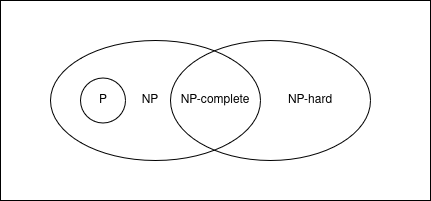
\includegraphics[width=0.9\textwidth]{./image/np_p_problems.png}
    \caption{Problem domains based on complexity}
    \label{fig:problem domains based on complexity}
\end{figure}
In above diagram, NP, NP-hard and NP-complete regions represent the non-polynomial time solvable problem categories explained earlier. P region represents the polynomial time solvable problems. Accordingly, based on our problem analysis, our research problem that was mapped to a boolean circuit, resides in NP region.\\ \\

% Implementation of boolean circuit
\section{Implementation of boolean circuit}
\subsection{Choice of technology}
As explained earlier, our research problem was mapped to a boolean circuit. And, that circuit was elaborated as five sequential algorithms, representing consecutive sub-sections of the entire boolean circuit. Since it is required to show that, those algorithms are convertible to a practical application in real world, a program was developed in our research.\\ \\
After analyzing potentially eligible programming languages and technologies, Python was selected as the programming language for implementing the program, representing five algorithms explained earlier. Because, in our analysis, it was noticed that Python has libraries containing built-in functions, executing the behavior of logic gates. In algorithms explained above, $AND, OR$ and $NOT$ logic gates are utilized. Therefore, when Python is used to implement above algorithms, it is not required to simulate the behavior of logic gates by us, since there are built-in Python functions. When developing the program as proof of concept, we used hard coded inputs. When executing the program for a new scenario, those inputs can be updated by editing the Python code.\\ \\
In addition, it is required to create mathematical combinations in $algorithm\ 3$, as explained earlier. In Python, there are libraries containing functions that support to create such combinations. Because, creating combinations is a problem of non-polynomial time complexity.\\
After compiling the Python code with a compiler, execution can be done in a console environment, such as Linux terminal or the console of a suitable Integrated Development Environment (IDE).\\

\subsection{Details on technology used for implementation}
Following table depicts the the version numbers and other specific details, regarding the technologies used to implement the program, as proof of concept.\\
\begin{table}[H]
    \renewcommand{\arraystretch}{1.5}
    \centering
    \begin{tabular}{|l|l|}
    \hline
    \textbf{Technology} & \textbf{Name and version} \\
    \hline
    Programming language & Python 3.7.0 \\
    \hline
    Compiler & GCC 7.2.0 \\
    \hline
    Library for logic gates & Sympy 1.2 \\
    \hline
    Library for mathematical combinations & Itertools bundled with Python 3.7.0 \\
    \hline
    Output console & Terminal of Ubuntu 22.04.4 LTS \\
    \hline
    \end{tabular}
    \caption{Technologies used to implement the proof of concept for algorithms}
    \label{tab:technologies used to implement the proof of concept for algorithms}
\end{table}

\subsection{Overview of the Python program}
This Python code has been designed to align with the definitions defined by us, earlier in this research, regarding concepts such as documents, groups of individuals, access control lists, classification of locations into three groups, time slots, meeting quorum etc. Therefore, it is recommended to be familiar with those definitions, before analyzing the Python code.\\ \\
Above algorithms are designed to accept the \textbf{individuals} present in \textbf{groups} in access control lists of documents, including the agenda, as input. Therefore, in this Python program, when defining the access control lists of documents, they should be defined in terms of singleton groups (i.e. individual person), instead of aggregate groups containing multiple individuals. But, $public$ group present in access control list of any document should not be resolved, since it is required to decide the eligible location for conducting the meeting. Following example depicts how access control lists should be defined in the Python program, for documents including the meeting agenda.\\ 
\begin{figure}[H] 
    \centering
    \begin{verbatim}
        doc1 = {"public"}
        doc2 = {"i_2", "i_3", "i_4", "i_5", "i_6"}
        agenda = {"public", "i_1", "i_2", "i_3", "i_4", "i_5"}
    \end{verbatim}
    \caption{Sample code snippet for defining access control lists of documents}
    \label{fig:sample code snippet for defining access control lists of documents}
\end{figure}
In addition, availability of individuals in different time slots, at different locations is stored in program using a dictionary. Sample section from this dictionary is depicted in the code snippet below.\\ 
\begin{figure}[H]  
    \centering
    \begin{verbatim}
        availability_dictionary = [
            {"person": "i_1", "slot": "slot1", "location": "onsite"},
            {"person": "i_1", "slot": "slot2", "location": "remote_private"},
            {"person": "i_2", "slot": "slot1", "location": "remote_public"}
        ]
    \end{verbatim}
    \caption{Sample code snippet for availability dictionary}
    \label{fig:sample code snippet for availability dictionary}
\end{figure}

Further, meeting quorum also should be defined as an input variable of integer type, in the program. Following example depicts how to define it, to mention the minimum number of participants required for conducting the meeting.\\ 
\begin{figure}[H]  
    \centering
    \begin{verbatim}
        meeting_quorum = 3
    \end{verbatim}
    \caption{Sample code snippet for defining meeting quorum}
    \label{fig:sample code snippet for defining meeting quorum}
\end{figure}    

When above mentioned inputs are defined by user, in the Python program, all required inputs are present in the code. There are five functions corresponding to five algorithms explained earlier. Each function has parameterized inputs. Some of those inputs are from inputs defined by user as explained above. In the program, these five functions are executed in sequential order, such that some outputs from initial functions are provided to later functions, as parameterized inputs. Following table depicts the name of Python function in code, corresponding to each algorithm explained earlier. In addition, output expected from execution of each function is also mentioned in the table.\\ 

\begin{table}[H]
    \renewcommand{\arraystretch}{1.5}  % Adjust row height for better readability
    \centering
    \begin{tabular}{|>{\centering\arraybackslash}p{0.5cm}|l|p{6cm}|}  % Use 'p{8cm}' for the right column to allow text wrapping
    \hline
    \textbf{\#} & \textbf{Function name in code} & \textbf{Output of the function} \\
    \hline
    1 & \texttt{doc\_analysis\_validation} & Validity of each individual for meeting, by document analysis \\
    \hline
    2 & \texttt{time\_slot\_and\_participant\_analysis} & Validity of each individual, in each time slot, by analyzing locations with expected privacy level for documents \\
    \hline
    3 & \texttt{meeting\_quorum\_analysis} & Meeting quorum satisfiability of each time slot, by validated participants \\
    \hline
    4 & \texttt{find\_earliest\_eligible\_slot} & Earliest privacy preserving time slot for the meeting \\
    \hline
    5 & \texttt{select\_meeting\_mode} & Meeting mode for each privacy preserving time slot identified \\
    \hline
    \end{tabular}
    \caption{Python functions corresponding to algorithms representing the boolean circuit (\# column represents the algorithm number)}
    \label{tab:python functions corresponding to algorithms representing the boolean circuit}
\end{table}
As it is described in problem analysis section, $algorithm\ 3$ contains an operation to create mathematical combinations. Since that operation has non-polynomial time complexity of $O(2^n)$, it has been implemented using $combinations$ function of $itertools$ library in Python. Because, there is no specific standard method to create combinations within polynomial time. Accordingly, it can be stated that, $itertools$ library was used by us, as an existing heuristic approach to create mathematical combinations.\\ 

When the program is compiled and executed, above mentioned outputs are displayed in the console, as boolean outputs. Some examples of such outputs are depicted in figures below.\\ 
\begin{figure}[H]  
    \centering
    \begin{verbatim}
        Participant validity by doc analysis:
        {'i_2': True, 'i_4': True, 'i_6': False, 'i_1': False, 
        'i_5': True, 'i_3': True}
    \end{verbatim}
    \caption{Output depicting participants validated by document analysis}
    \label{fig:output depicting participants validated by document analysis}
\end{figure} 
In above output, $true$ or $false$ states whether each individual is validated by analyzing access control lists of documents, including the agenda document as well. If an individual has no access to all the documents discussed in the meeting, particular individual will be marked as $false$.\\ 

\begin{figure}[H]  
    \centering
    \begin{verbatim}
        Time Slot: slot1
            slot1_i_2_eligibility: True
            slot1_i_4_eligibility: True
            slot1_i_6_eligibility: False
            slot1_i_1_eligibility: False
            slot1_i_5_eligibility: False
            slot1_i_3_eligibility: True
    \end{verbatim}
    \caption{Output depicting eligibility of each participant in a time slot, based on analysis of location with required level of privacy for documents}
    \label{fig:output depicting eligibility of each participant in a time slot, based on analysis of location with required level of privacy for documents}
\end{figure} 
Above section of output displays the eligibility of each individual to attend the meeting, in each time slot. To decide the eligibility of an individual, in a certain time slot, algorithm analyzes the location of that individual, with the expected level of privacy for documents in the meeting.\\ 

\begin{figure}[H]  
    \centering
    \begin{verbatim}
        Slot: slot1 - Quorum Satisfiability: True
        Slot: slot2 - Quorum Satisfiability: True
        Slot: slot3 - Quorum Satisfiability: True
        Slot: slot4 - Quorum Satisfiability: False
    \end{verbatim}
    \caption{Output depicting meeting quorum satisfiability of each time slot}
    \label{fig:output depicting meeting quorum satisfiability of each time slot}
\end{figure} 
Above section of output states whether each time slot satisfies the meeting quorum, by having enough number of participants at privacy preserving locations, according to the expected level of privacy for documents in the meeting.\\ 

\begin{figure}[H]  
    \centering
    \begin{verbatim}
        Slot 1 eligibility as earliest slot: True
        Slot 2 eligibility as earliest slot: False
        Slot 3 eligibility as earliest slot: False
        Slot 4 eligibility as earliest slot: False
    \end{verbatim}
    \caption{Output depicting earliest privacy preserving time slot for the meeting}
    \label{fig:output depicting earliest privacy preserving time slot for the meeting}
\end{figure} 
In above section of output, that depicts the earliest quorum satisfying time slot for meeting, only one slot is supposed to have $true$ value. Because, once after identifying a quorum satisfying time slot, among all the time slots arranged in sequential order, algorithm marks all other time slots after the identified time slot as, $false$. If no quorum satisfying time slot is present, all time slots will be marked as $false$, since it is impossible to identify an earliest eligible time slot.\\ 

\begin{figure}[H]  
    \centering
    \begin{verbatim}
        Slot1:
            Eligibility online: False
            Eligibility hybrid: False
            Eligibility onsite: True
    \end{verbatim}
    \caption{Output depicting meeting mode for each privacy preserving time slot identified}
    \label{fig:output depicting meeting mode for each privacy preserving time slot identified}
\end{figure} 
Above section of output depicts the eligible meeting mode for conducting the meeting, in each time slot. Algorithm is designed such that more than one meeting mode cannot be activated (cannot be $true$) for a particular time slot. If a time slot is not suitable to conduct a privacy preserving meeting with equal or more number of participants than the meeting quorum value, all three meeting modes will get $false$ for that time slot, to display that meeting should not be conducted in particular time slot.\\ \\
In overall, above overview describes the inputs, outputs and behavior of the Python program, implemented as proof of concept, associated with algorithms explained earlier. In our research, those algorithms are converted to the Python code such that maximum possible time complexities identified do not get exceeded.\\ \\

\subsection{Application of the Python program}
Python program developed by us to implement the boolean circuit is available in GitHub (\cite{Thejana2025sympy_solver}). There are comments in the program, for easily understanding its content. It can be cloned and executed by anyone in an environment supporting Python 3.7.0 version. Input sections can be edited during execution, to observe the variation of result. Variation of results in different scenarios is explained with more details in the section below. \\ \\

% Result of pragram execution
\section{Result of program execution}
\subsection{Overview of the result}
As explained in code overview, program contains three inputs including the access control lists of documents, availability details of individuals in time slots (availability dictionary) and the meeting quorum. When these inputs are edited and program is executed, it can be observed that output changes. Possible outputs of five algorithms contained in the program can be summarized as below.\\ 
\begin{figure}[H]
    \centering
    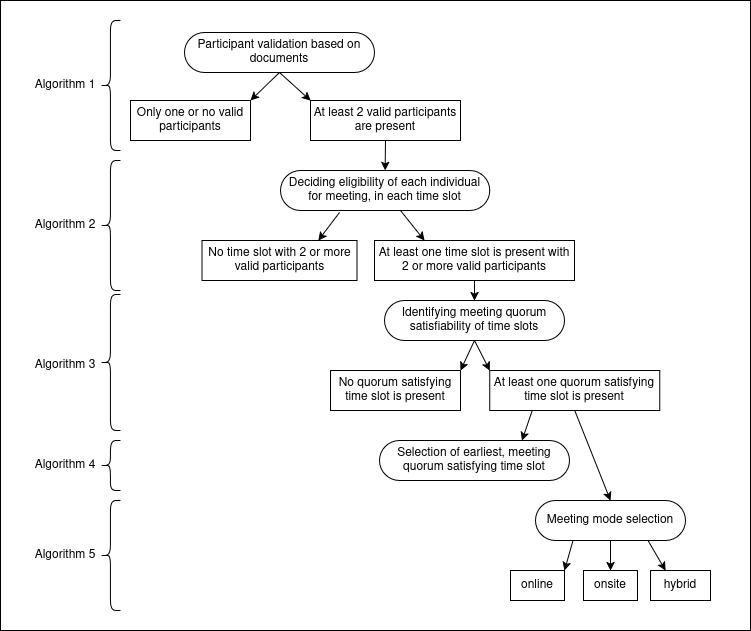
\includegraphics[width=0.9\textwidth]{./image/workflow_execution_result.png}
    \caption{Possible results of program execution}
    \label{fig:possible results of program execution}
\end{figure}

In addition, though each negative output shows the end of process in above diagram for simplicity, when considering the boolean circuit, processing does not stop abruptly in that manner. Instead of stopping, after a reaching a certain negative output, all remaining outputs also become negative ($false$), in boolean circuit. Three negative outputs identified in the program execution are listed below.
\begin{itemize}
    \item $Algorithm\ 1$: Only one or no valid participants
    \item $Algorithm\ 2$: No time slot with 2 or more valid participants
    \item $Algorithm\ 3$: No quorum satisfying time slot is present
\end{itemize}
Accordingly, for reaching a positive output which means that meeting can be conducted, none of above three negative outputs should be encountered in program execution. In other words, if program approaches at least one negative output among above three, then it is impossible to conduct the particular meeting as a privacy preserving meeting.\\ \\
In our research, we have considered variation of output with changes in input, to check whether they validate our hypothesis. After breaking down possible outputs of five algorithms as depicted above, sections of output supporting to validate the hypothesis were analyzed. Here, it is needed to note that, some sections of output are not required to validate the hypothesis. Such sections were introduced by us, as additional contributions, to enhance the quality of research outcome.\\ \\

\subsection{Analytical investigation of the result}
When $algorithm\ 1$ is considered, its output shows whether each individual is allowed to discuss all documents included in the meeting. In this case, we consider having at least two valid participants as the positive output, since at least two participants are required for conducting a meeting. This decision is made by analyzing the access control lists of documents associated with the meeting, including the meeting agenda. Following flow chart depicts the process within $algorithm\ 1$, to generate the expected output.\\ \\
\begin{figure}[H]
    \centering
    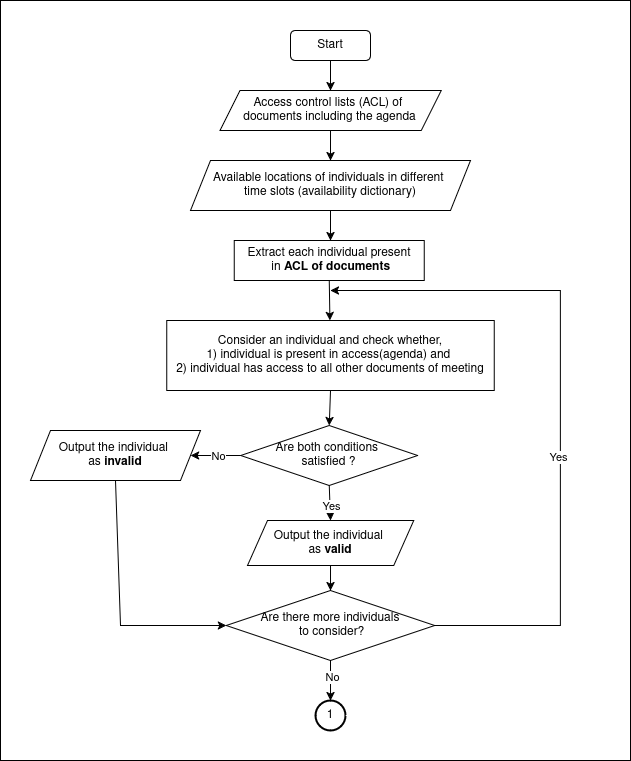
\includegraphics[width=0.9\textwidth]{./image/algo01_result_analysis.png}
    \caption{Participant validation by document analysis in $algorithm\ 1$}
    \label{fig:Participant validation by document analysis in algorithm 1}
\end{figure}
Output of $algorithm\ 2$ shows whether each individual is allowed to discuss all documents of the meeting, in each time slot. As discussed in problem analysis section, to make this decision, program checks whether at least one private document is present in meeting. If at least one private document is present, an individual present at a public location in a certain time slot is not allowed to attend this meeting, in that time slot. However, whether a document is private or public (by presence of $"public"$ group), is stated in the access control list of the document. Following flow chart depicts the process within $algorithm\ 2$, to generate the expected output.\\ \\
\begin{figure}[H]
    \centering
    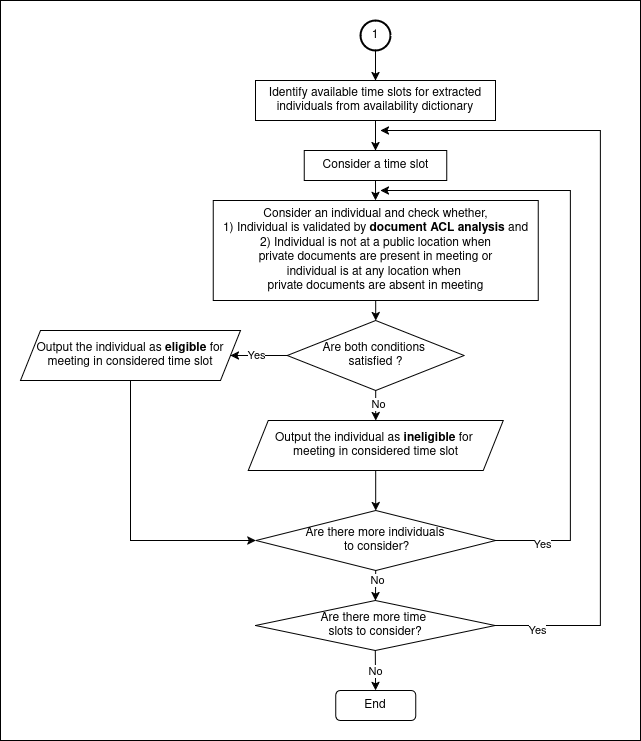
\includegraphics[width=0.9\textwidth]{./image/algo02_result_analysis.png}
    \caption{Deciding eligibility of each individual in $algorithm\ 2$}
    \label{fig:Deciding eligibility of each individual in algorithm 2}
\end{figure}
By observing these two segments of flow chart connected by a connector, it can be understood that access control lists of documents play a vital role as an essential input, to decide the eligible meeting participants. It means that, \textbf{"Meeting participant selection is primarily dominated by the access control lists of the documents presented including meeting agenda"} expression is validated by analyzing the process within $algorithm\ 1$ and $algorithm\ 2$ collectively, as in above flow chart segments.\\ \\ 
After identifying the eligibility of each individual to attend the meeting in each time slot, next result expected from the program is whether each time slot satisfies the meeting quorum. Though meeting quorum is not relevant to privacy of meeting data, it is an important feature in meeting domain, to determine whether minimum required number of participants is present in meeting. In our research, $algorithm\ 3$ enhances the quality of research outcome, by checking whether each time slot satisfies the meeting quorum, with enough eligible meeting participants, for a privacy-preserved meeting. In other words, our requirement is to satisfy the meeting quorum, without violating the privacy of meeting data. Accordingly, identification of quorum satisfying time slots as well, depends on access control lists of documents of the meeting. Meeting quorum value should be be defined by user as an input, in program.\\ \\
After identifying quorum satisfying time slots, it is required to identify the earliest one among them. If there are more than one quorum satisfying time slots, $algorithm\ 4$ selects the earliest one among them. If only one time slot satisfies the meeting quorum, it becomes the earliest one. However, since $algorithm\ 4$ depends on $algorithm\ 3$, it can be stated that, outcome of $algorithm\ 4$ indirectly depends on access control lists of documents. Result of $algorithm\ 3$ and $alogorithm\ 4$ do not support to validate the hypothesis, since these two algorithms focus on quality related attributes, rather than privacy of meeting data. \\ \\
After quorum satisfying time slots are identified by $algorithm\ 3$, $algorithm\ 5$ decides the privacy-preserving meeting mode for each of such time slots, by analyzing the locations of eligible participants. Every quorum satisfying time slot belongs to one meeting mode out of three modes---onsite, online and hybrid. Essential input required to generate the meeting mode of a time slot as output, is the available location of every eligible participant, in the particular time slot. The logic for selecting the meeting mode is discussed in "meeting mode selection" (\ref{sec:logic_for_selecting_the_meeting_mode}) section of problem analysis. \\ \\
Accordingly, since program decides the meeting mode of a quorum satisfying time slot by analyzing locations of eligible meeting participants, \textbf{"the choice of meeting mode depends on the participants’ locations."} phrase of hypothesis is validated by $algorithm\ 5$.

\subsection{Relationship between input and the result}
To observe the way how relationship between input and output supports the hypothesis as explained above, a sample data set has been designed. That sample data set is available in GitHub (\cite{Thejana2025CircuitResultAnalysis}). The data set has been designed such that availability dictionary is same for all scenarios. Only access control lists of documents and meeting quorum are changed, for observing the variation of output. There are comments in the data set, for applying data in the program conveniently, by a user. However, since our data set is not an exhaustively large data set, anyone can extend this data set to include more scenarios, and execute the program to observe how result changes from scenario to scenario. To validate the analytical investigation of result presented by us above, it is required to observe whether results align with the hypothesis, in each execution. \\ \\


% Evaluation
\section{Evaluation}
\indent \par In our research, initially entities in privacy-preserving meeting context were defined formally, using standard notations. After that, using those formal definitions as the foundation, research problem was mapped to a boolean circuit for analyzing it easily. Specially for analyzing the complexity of the problem, boolean circuit was depicted in algorithmic representation. Time complexity of the problem was calculated by considering the quantity of input variables and loops present in that algorithmic representation.\\
\par As the evaluation procedure, we implemented algorithmic representation of circuit using Python. And then output of the Python program was manually checked, by setting the inputs. Those results were cross-validated with the output of algorithm, to ensure that implemented Python program aligns with the algorithm. Then possible results of the execution of Python program regarding selection of eligible participants, eligible time slot and eligible meeting mode, were discussed. And, we highlighted when a negative output showing that a privacy-preserved meeting is not possible will be delivered. These results were discussed, considering the segments of the algorithm, for aligning with the algorithmic level analysis of the problem.\\
\par Later, an analytical investigation was conducted on results obtained by execution of Python program. This investigation is for showing how segments of algorithm contribute to validate the hypothesis built in the beginning of research. Further a sample data set was introduced to observe the variation of results in Python program execution. Since we have published our Python program implementation and this sample dataset in GitHub, anyone can test to check the validity.\\
\par Using existing public platforms such as Google-API, a simple system was implemented to prove that privacy-preserved meeting organization is practically viable. Therefore, it can be confirmed that, this is not limited to a theoretical concept. But, this is a practical approach, which can be improved further in future, to organize privacy-preserved meetings in practical context.\\
\par Accordingly, it is observed that there is a flow of logically related steps in this research, which started from basic set of definitions, and was developed up to a practical application that can be tested by anyone. Therefore, it can be determined that, there is no mismatch in intermediate steps. Hence, in overall, it can be concluded that, contribution by this research is valid and acceptable.\\
\begin{figure}[H]
    \centering
    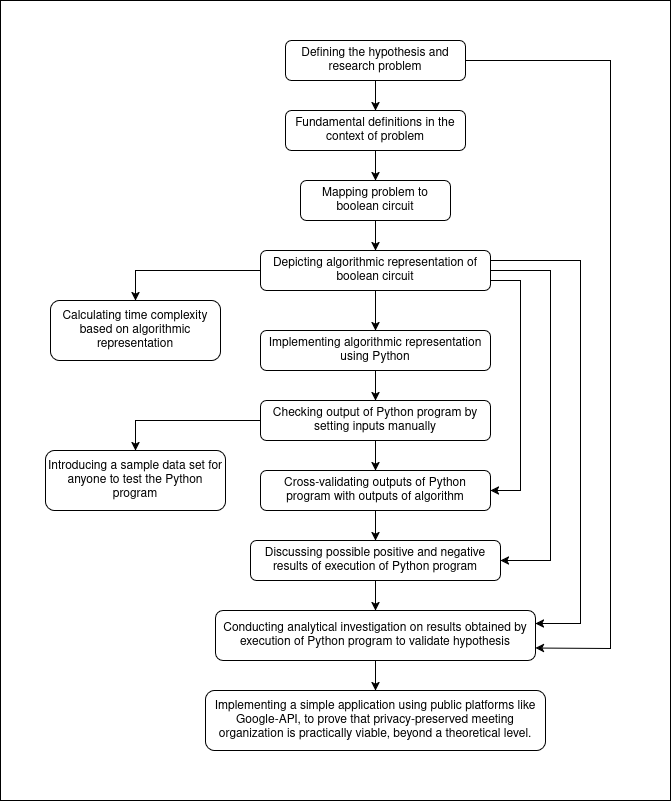
\includegraphics[width=0.9\textwidth]{./image/evaluation_flow.png}
    \caption{Flow of logically related steps in research}
    \label{fig:Flow of logically related steps in research}
\end{figure}

% Conclusion
\section{Conclusion}
\indent \par The research question was developed based on a hypothesis. Hypothesis was developed including the factors affecting the privacy of meeting. After that, above explained flow of interrelated steps was followed, to prove that hypothesis is correct.\\
\par As validity of the research approach can be proven by logically related nature of steps, which started from initial fundamental definitions, it can be concluded that, this research has contributed to privacy-preserved meeting organization successfully. And, since this is only an initiative approach to concern the privacy of meeting data, more research can be conducted in future, via the future paths highlighted as future work.\\

% Limitations and future work
\section{Limitations and future work}
\indent \par Since this research considers only a provided set of documents to organize a meeting, it is not possible to suggest how those documents can be divided to discuss in two or more meetings, in case they cannot be discussed in same meeting. It is an optimization problem, for which a heuristic approach will be required, after a thorough analysis. That research path is one future work.\\
\par Another future work is to consider privacy preserved meeting organization problem with various additional constraints such as meeting precedence, number of onsite physical locations available. Because, in related work, there are constraint optimization research that have concerned such additional constraints other than the main research problem (\cite{bofill2022}).\\
\par In our research, meeting quorum is considered as an additional constraint, in which it is checked whether minimum required number of participants can attend the meeting, in a particular time slot. But, this constraint can be improved further to consider the minimum number of participants including essentially required participants as well, such that minimum number must definitely contain those participants. It is another possible future work in our research.\\
\par And, we have developed a Google-APIs based simple application to prove the usability and practical applicability of a solution for privacy-preserved meeting organization. In future, someone can develop a more advanced application with advanced features, for organizing privacy preserved meetings.\\
\par Therefore, it can be said that, our research is an initiative in a less-observed research area, associated with privacy-preserved meeting organization.\\

%Appendix
\newpage
\section{Appendix}
\subsection{Maximum value of $n \text{C} r$} \label{proof: maximum value of ncr when n is n/2}
\text{The following proof shows that } $n \text{C} r$ \text{ is maximum when } $r = \frac{n}{2}$ \text{ or } $r \approx \frac{n}{2}$.

\[ \binom{n}{r} = \frac{n!}{(n-r)!r!} \]
\[ \binom{n}{r+1} = \frac{n!}{(r+1)!(n-r-1)!} \]
\[ \frac{\binom{n}{r}}{\binom{n}{r+1}} = \frac{\frac{n!}{(n-r)!r!}}{\frac{n!}{(r+1)!(n-r-1)!}} \]
\[ \frac{\binom{n}{r}}{\binom{n}{r+1}} = \frac{\frac{n!}{(n-r-1)!(n-r)r!}}{\frac{n!}{r!(r+1)(n-r-1)!}} \]
\[ \frac{\binom{n}{r}}{\binom{n}{r+1}} = \frac{\frac{n!}{(n-r-1)!(n-r)r!}}{\frac{n!}{r!(r+1)(n-r-1)!}} = \frac{r+1}{n-r} \]

\text{Therefore, when } $\frac{\binom{n}{r}}{\binom{n}{r+1}} < 1$, 
\[ \quad \frac{r+1}{n-r} < 1 \]
\[ \quad r+1 < n-r \]
\[ \quad r < \frac{n-1}{2} \]\\

 \text{When } $\frac{\binom{n}{r}}{\binom{n}{r+1}} = 1$, 
\[ \quad \frac{r+1}{n-r} = 1 \]
\[ \quad r+1 = n-r \]
\[ \quad r = \frac{n-1}{2} \]

\text{When } $\frac{\binom{n}{r}}{\binom{n}{r+1}} > 1$, 
\[ \quad \frac{r+1}{n-r} > 1 \]
\[ \quad r+1 > n-r \]
\[ \quad r > \frac{n-1}{2} \]

According to definition of $n \text{C} r$ in mathematics, $n$ is a positive integer $(n \in \mathbb{Z}^+)$, $r$ is a non-negative integer $(r \in (\mathbb{Z}^+ \cup \{0\}))$, and $n \geq r$ (\cite{uow168693}, \cite{newcastle_permutations_combinations}).\\
$\therefore$ For $r = \frac{n-1}{2}$ to be satisfied, $n$ must be an odd integer.\\ \\
When $n$ is an odd integer, the variation of the magnitude of $n \text{C} r$ can be graphically depicted as below, based on the above calculations.\\ \\
\begin{figure}[H]
    \centering
    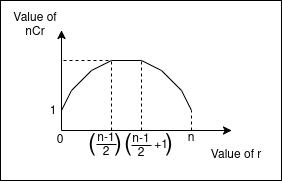
\includegraphics[width=0.7\textwidth]{./image/ncr_for_odd_n.png}
    \caption{Variation of $n \text{C} r$ for different $r$ values, when $n$ is an odd integer}
    \label{fig:Variation of nCr for different r values, when n is an odd integer}
\end{figure}
By analyzing that graph, it can be proven that $n \text{C} r$ is maximum when $r \approx \, \frac{n}{2}$. Because, $\frac{n}{2}$ is not an integer, when $n$ is odd. ($\frac{n}{2} \approx \frac{n-1}{2}$ and $\frac{n}{2} \approx \left(\frac{n-1}{2}\right) + 1$)\\ \\
When considering values from 0 to $n$ for $r$, in $n \text{C} r$, the following symmetric pattern is observed.\\
\[ n \text{C} 0 = \binom{n}{0} = \frac{n!}{(n-0)!0!} \]
\[ \binom{n}{n-0} = \frac{n!}{(n-0)!(n-(n-0))!} = \frac{n!}{(n-0)!0!} \]
\[ \therefore \binom{n}{0} = \binom{n}{n-0} \]\\

\[ n \text{C} 1 = \binom{n}{1} = \frac{n!}{(n-1)!1!} \]
\[ \binom{n}{n-1} = \frac{n!}{(n-1)!(n-(n-1))!} = \frac{n!}{(n-1)!1!} \]
\[ \therefore \binom{n}{1} = \binom{n}{n-1} \]\\

\[ n \text{C} 2 = \binom{n}{2} = \frac{n!}{(n-2)!2!} \]
\[ \binom{n}{n-2} = \frac{n!}{(n-2)!(n-(n-2))!} = \frac{n!}{(n-2)!2!} \]
\[ \therefore \binom{n}{2} = \binom{n}{n-2} \]\\

It means that, $\binom{n}{r} = \binom{n}{n-r}$. But, in that pattern, when $n$ is an even number, and $r = \frac{n}{2}$ is reached, following observation is noticed.\\
\[ r = \frac{n}{2} \]
\[ n - r = n - \frac{n}{2} = \frac{n}{2} \]
\[ \therefore \binom{n}{\frac{n}{2}} = \binom{n}{n - \frac{n}{2}} \]
It means that, value of $\binom{n}{r}$ when $r = \frac{n}{2}$ is available only for $r = \frac{n}{2}$. Because, $r = n - r$.\\
Based on previous inequalities, following relationships are present for even $n$ values. \\
When $\frac{\binom{n}{r}}{\binom{n}{r+1}} < 1$, 
\[ \quad r < \frac{n-1}{2} \]
Since $\frac{n-1}{2} < \frac{n}{2}$, 
\[ \quad r < \frac{n-1}{2} < \frac{n}{2} \]\\
When $\frac{\binom{n}{r}}{\binom{n}{r+1}} > 1$, 
\[ \quad r > \frac{n-1}{2} \]
When $n$ is an even integer, the variation of the magnitude of $n \text{C} r$ can be graphically depicted as below, based on the above factors.\\ \\
\begin{figure}[H]
    \centering
    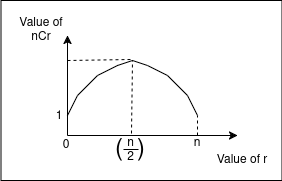
\includegraphics[width=0.7\textwidth]{./image/ncr_for_even_n.png}
    \caption{Variation of $n \text{C} r$ for different $r$ values, when $n$ is an even integer}
    \label{fig:Variation of nCr for different r values, when n is an even integer}
\end{figure}
In ensemble, it is concluded that, $\binom{n}{r}$ is maximum when $r = \frac{n}{2}$ or $r \approx \frac{n}{2}$.

\subsection{Value of $\binom{n}{\frac{n}{2}}$ for large $n$ values} \label{proof: time complexity of nc(n/2)}

\[ n! \approx \sqrt{2 \pi n} \left( \frac{n}{e} \right)^n \quad \text{(By Stirling's approximation, \cite{hosch2025stirlings})} \quad \Rightarrow \quad 1 \]
\[ \therefore \quad \left( \frac{n}{2} \right)! \approx \sqrt{\frac{2 \pi n}{2}} \left( \frac{n}{2e} \right)^{n/2} \quad \Rightarrow \quad 2 \]
\[ \binom{n}{\frac{n}{2}} = \frac{n!}{(\frac{n}{2})! (n - \frac{n}{2})!} = \frac{n!}{(\frac{n}{2})! (\frac{n}{2})!} \text{ (By nCr combination)} \]
\[ \frac{n!}{(\frac{n}{2})! (\frac{n}{2})!} \approx \frac{\sqrt{2 \pi n} \left( \frac{n}{e} \right)^n}{\sqrt{\frac{2 \pi n}{2}} \left( \frac{n}{2e} \right)^{\frac{n}{2}} \cdot \sqrt{\frac{2 \pi n}{2}} \left( \frac{n}{2e} \right)^{\frac{n}{2}}} \quad \text{(By 1 and 2)} \]
\[ \frac{n!}{(\frac{n}{2})! (\frac{n}{2})!} \approx \frac{\sqrt{2 \pi n} \left( \frac{n}{e} \right)^n}{\pi n \left( \frac{n}{2e} \right)^n} \]
\[ \frac{n!}{(\frac{n}{2})! (\frac{n}{2})!} \approx \sqrt{2 \pi n} \cdot \frac{n^n}{e^n} \cdot \frac{2^n e^n}{\pi n n^n} \]
\[ \therefore \quad \frac{n!}{(n/2)! (n/2)!} \approx \sqrt{\frac{2}{\pi n}} \cdot 2^n \]
\[ \text{It means that, } \quad \binom{n}{\frac{n}{2}} \approx \sqrt{\frac{2}{\pi n}} \cdot 2^n \]
\[ \therefore O\binom{n}{\frac{n}{2}} \approx O(\frac{2^n}{\sqrt{n}}) \]

\subsection{Value of $\binom{n}{\frac{n-1}{2}}$ for large $n$ values} \label{proof: time complexity of nc((n-1)/2)}

In $\binom{n}{\frac{n-1}{2}}$, when $2m+1$ is substituted for $n$, and $m$ is substituted for $\frac{n-1}{2}$,
\[ \binom{n}{\frac{n-1}{2}} = \binom{2m+1}{m} \]
\[ \binom{2m+1}{m} = \frac{(2m+1)!}{(m+1)!m!} \text{ (By nCr combination)} \Rightarrow \quad 1 \]

\[ \binom{2m+1}{m+1} = \frac{(2m+1)!}{(m+1)!m!} \text{ (By nCr combination)} \Rightarrow \quad 2 \]
\[ \frac{(2m+1)!}{(m+1)!m!} = \frac{(2m+1)!(2m+2)}{(m+1)!m!(2m+2)} \]
\[ \frac{(2m+1)!(2m+2)}{(m+1)!m!(2m+2)} = \frac{(2m+2)!}{(m+1)!m!2(m+1)} \]
\[ \frac{(2m+2)!}{(m+1)!m!2(m+1)} = \frac{(2m+2)!}{2.(m+1)!(m+1)!} \]
\[ \frac{(2m+2)!}{2.(m+1)!(m+1)!} = \frac{1}{2}.\frac{(2m+2)!}{(m+1)!(m+1)!} \]
\[ \frac{1}{2}.\frac{(2m+2)!}{(m+1)!(m+1)!} = \frac{1}{2}.\binom{2m+2}{m+1}  = \frac{1}{2}.\binom{2(m+1)}{m+1} \Rightarrow \quad 3 \] \\

By considering 2 and 3,
\[ O\binom{2m+1}{m+1} = O\binom{2(m+1)}{m+1} \] \\
By 1 and 2,
\[ \binom{2m+1}{m+1} = \frac{(2m+1)!}{(m+1)!m!} = \binom{2m+1}{m} \]
\[ \therefore O\binom{2m+1}{m+1} = O\binom{2m+1}{m} \]
\[ O\binom{2m+1}{m} = O\binom{2(m+1)}{m+1} \] \\

By above proof \ref{proof: time complexity of nc(n/2)},
\[ O\binom{2(m+1)}{m+1} \approx O(\frac{2^{2(m+1)}}{\sqrt{2(m+1)}}) \]
When 2(m+1) is considered as an integer $n$,
\[ O(\frac{2^{2(m+1)}}{\sqrt{2(m+1)}}) \approx O(\frac{2^n}{\sqrt{n}}) \]




%List of References 
\newpage
\addcontentsline{toc}{section}{List of References }
\section*{\begin{LARGE} List of References  \end{LARGE} }
\printbibliography

\end{document}

